%% Put these somewhwere:

\XXX{use svalue(g), spacing to give some breathing room in a ggroup}

\XXX{something like ggroup(cont=w,spacing=10); svalue(g)=10}

\XXX{include listing data frame, listing variables by type}

\XXX{relationship with the toolkits

\XXX{getToolkitWidget, add method, ... only with RGtk2 (rJava?), only some widgets}}



%% gWidgets introduction
 
\newcommand{\ONLYIN}[1]{[only in #1]}

\chapter{\pkg{gWidgets}: Overview}
\label{sec:overview}

%% Overview of gWidgets

% ML: do we really want to discuss the unsupported rJava backend?
% I am also confused about gWidgetsWWW - is it an implementation or
% something that just resembles the gWidgets API?

% JV, I will drop rJava, put in gWidgetsQt, and make brief mention of gWidgetsWWW

The \pkg{gWidgets} package provides a toolkit-independent interface
for the \R\/ user to program graphical user interfaces from within
R. Although the package provides much less functionality than using a
native toolkit interface, \pkg{gWidgets} can be used to create
moderately complex GUIs quickly and easily using a programming
interface that is simpler and more familiar to the \R\/ user.

Figure~\ref{fig:gWidgets-three-oses} demonstrates the portability of
\pkg{gWidgets} commands, as it shows realizations on different
operating systems and with different graphical toolkits.

\begin{figure}
  \centering
  \begin{tabular}{ll}
    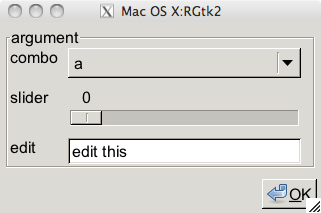
\includegraphics[width=0.45\textwidth]{ex-33-macosx-rgtk2} &
    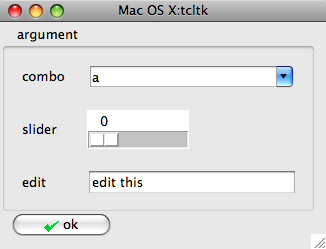
\includegraphics[width=0.45\textwidth]{fig-gWidgets-ex-33-tlctk}\\
    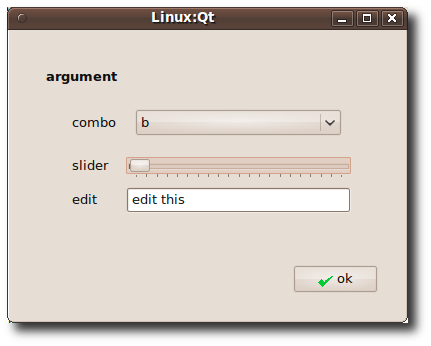
\includegraphics[width=0.45\textwidth]{ex-33-linux-qt} &
    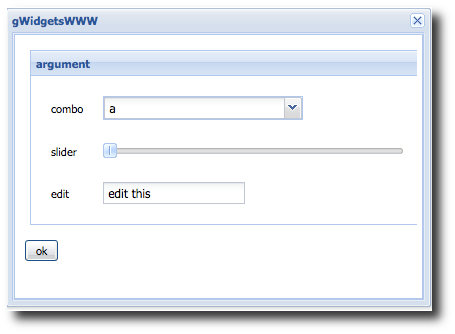
\includegraphics[width=0.45\textwidth]{ex-33-gWidgetsWWW}
  \end{tabular}
  \caption{The \pkg{gWidgets} package works with different operating
    systems and different GUI toolkits. This shows, the same code using the
    \pkg{RGtk2}, \pkg{tcltk}, \pkg{qtbase} packages for a toolkit. Additionally,
    the \pkg{gWidgetsWWW} package is used in the lower right figure.}
  \label{fig:gWidgets-three-oses}
\end{figure}

% %% Make figure -- work on layout here
% \XXX{Do mac, windows}
% \begin{figure}
%   \centering
%   \begin{tabular}{lccc}
%     & \pkg{RGtk2} & \pkg{tcltk} & \pkg{rJava} 
%     \\
%     L &
%     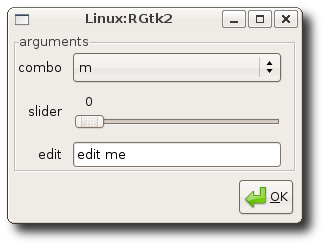
\includegraphics[width=0.3\textwidth]{ex-33-linux-rgtk2.png} &
%     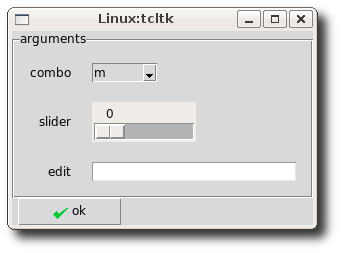
\includegraphics[width=0.3\textwidth]{ex-33-linux-tcltk} &
%     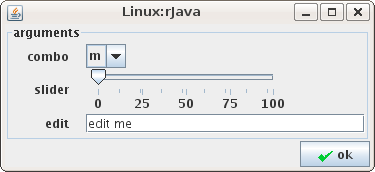
\includegraphics[width=0.3\textwidth]{ex-33-linux-rJava} 
%     \\
%     W &
%     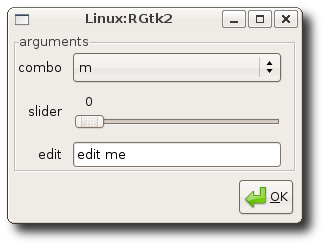
\includegraphics[width=0.3\textwidth]{ex-33-linux-rgtk2} &
%     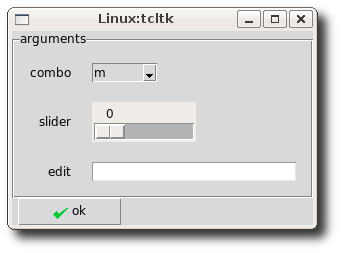
\includegraphics[width=0.3\textwidth]{ex-33-linux-tcltk} &
%     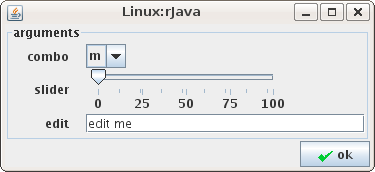
\includegraphics[width=0.3\textwidth]{ex-33-linux-rJava} 
%     \\
%     Mac &
%     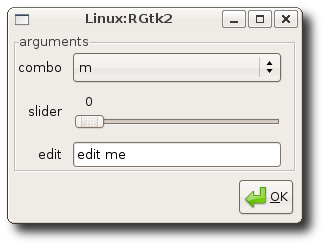
\includegraphics[width=0.3\textwidth]{ex-33-linux-rgtk2} &
%     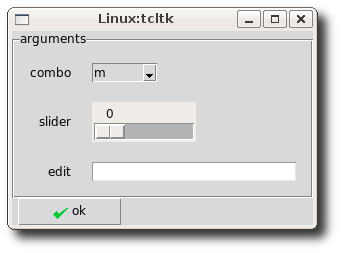
\includegraphics[width=0.3\textwidth]{ex-33-linux-tcltk} &
%     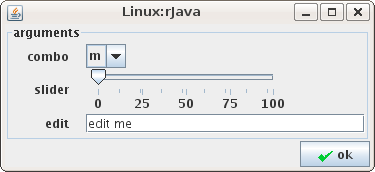
\includegraphics[width=0.3\textwidth]{ex-33-linux-rJava}
%   \end{tabular}
%   \caption{The \pkg{gWidgets} package works with different operating systems and different GUI toolkits. This shows the combination of \code{linux}, \code{Mac OS X (10.5)} and \code{Windows XP} and the packages \pkg{RGtk2}, \pkg{tcltk}, and \pkg{rJava}}
%   \label{fig:three-oses-three-toolkits}
% \end{figure}


% \begin{figure}
%   \centering
%   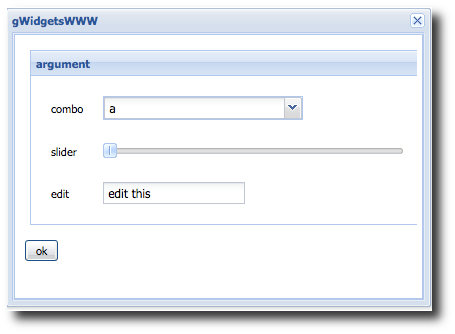
\includegraphics[width=.45\textwidth]{ex-33-gWidgetsWWW}
%   \caption{A GUI shown using \pkg{gWidgetsWWW}.}
%   \label{fig:gWidgetsWWW-same-gui}
% \end{figure}





\section{Constructors}
\label{sec:constructors}

We begin with some sample \pkg{gWidgets} commands that set up a basic
interface allowing a user to input some test. The first line loads the
package, the others will be described later.

\begin{Schunk}
\begin{Sinput}
 require(gWidgets)
 options(guiToolkit="RGtk2")
 w <- gwindow("Text input example", visible=FALSE)
 g <- ggroup(container=w)
 l <- glabel("Your name:", cont=g)
 e <- gedit("", cont=g)
 b <- gbutton("Click", cont=g, handler=function(h,...) {
   msg <- sprintf("Hello %s", svalue(e))
   cat(msg, "\n")
 })
 visible(w) <- TRUE
\end{Sinput}
\end{Schunk}


This example defines five different widgets, a window, a box
container, a label, a single-line, text edit area and a button. These
GUI objects are produced by constructors.


\pkg{gWidgets} most constructors have the following form: 
\begin{Schunk}
\begin{Sinput}
 gname(arguments, handler = NULL, action = NULL, 
       container = NULL,...,toolkit=guiToolkit())
\end{Sinput}
\end{Schunk}
where the \code{arguments} vary depending on the object being made. 

In the above, we see that the \code{gwindow} constructor, for a
top-level window, has two arguments passed in, an unamed one for a
window title and a value for the \code{visible} property. Whereas the
\code{ggroup} constructor takes all the default arguments except for
the parent container.

%% container
A top-level window does not have a parent container, but other GUI
components do. In \pkg{gWidgets}, for the sake of portability, the
parent container is passed to the widget constructor through the
\args{container} argument, as it done in all the other constructors.
This argument name can always be abbreviated \args{cont}. This defines
the GUI layout, a topic taken up in
Chapter~\ref{sec:gWidgets-Containers}.

%% toolkit
The \args{toolkit} argument is usually not specified. It is there to
allow the user to mix toolkits within the same \R\/ session, but in
practice can cause problems due to competing event loops. The default
call \function{guiToolkit} which will query the user for a choice of
toolkit, if one has not been specified and a choice is available. In
our example we have the call
\begin{Schunk}
\begin{Sinput}
 options(guiToolkit="RGtk2")
\end{Sinput}
\end{Schunk}
to explicitly set the toolkit, thereby avoiding being asked when the
\code{toolkit} argument is evaluted.



%% return value
The constructors produce three general types of objects: containers,
such as the top level window \code{w} and the box container \code{g}
(Table~\ref{tab:gWidgets-container-constructors}); components, such as
a label \code{l}, the edit area \code{e} or the button \code{b}.
(Table~\ref{tab:gWidgets-control-widgets} and
Table~\ref{tab:gWidgets-compound-widgets}) show the basic and compound
widgets.)  dialogs.



%% container argument
% ML: this has already been well explained in preceeding chapters
% A GUI consists of a heiarchical nesting of containers. Each container
% may contain contain controls or additional containers. In a GUI,
% except for top-level windows (including dialogs), every component and
% container is the child of some parent container. 

% ML: This sounds to me that it is a detail of specific toolkit implementations
% The package does not implement layout managers. Rather, in
% the construction of a widget in \pkg{gWidgets}, the
% \meth{add} method for the parent container is called with the new
% object as an argument and the values passed through the \args{...}
% argument as arguments.  


% We remark that not all the toolkits (e.g., \pkg{RGtk2}, \pkg{qtbase})
% require one to combine the construction of an object with the
% specification of the parent container. We don't illustrate this, as
% the resulting code is not cross-toolkit.

% % toolkit argument
% The \code{toolkit} can be specified at time of construction allowing
% tookits, in theory, to be mixed. Otherwise, the \code{guiToolkit}
% function returns the currently selected toolkit, or queries for one if
% none is selected.  Constructors dispatch on the \code{toolkit} value
% to call the appropriate constructor in the toolkit implementation. The
% return value from the toolkit's constructor is kept in the
% \code{widget} component.

\section{Methods}


In addition to creating a GUI object, a constructor also returns a
useful \R\/ object. Except for modal dialog constructors, this is an
S4 object of a certain class containing two components: \code{toolkit}
and \code{widget}. (Modal dialogs do not return an
object, as the dialog will be destroyed before the
constructor returns. Instead, their constructors return values reflecting the
user response to the dialog.)


GUI objects have a state determined by one or more of their
properties. In \pkg{gWidgets} many properties are set at the time of
construction. However, there are also several generic methods defined
for \pkg{gWidgets} objects. ~\footnote{
  In \pkg{gWidgets} constructors are generic functions that dispatch
  down to the toolkit implementation after considering the
  \args{toolkit} argument. For example, \function{gbutton} calls
  \function{.gbutton}, defined in the toolkit implementation. This in
  turn calls a GUI toolkit command, such as
  \function{gtkButton}. This is then placed as a slot in an S4 object
  which in turn is placed in another S4 object, which is the GUI
  object available to interact iwth. As such, in \pkg{gWidgets}, generic
  methods also have a double dispatch when called.
 
  The actual class of
  the S4 object returned by the first constructor is (mostly) not
  considered, but when we refer to methods for an object, we gloss
  over this double dispatch and think of it as a single dispatch. This
  design allows the toolkit packages the freedom to implement their
  own class structure.
}

%% s3 generics
Depending on the class of the object, the \pkg{gWidgets} package provides methods
for the familiar S3 generics \generic{[}, \generic{[$<$-},
\generic{dim}, \generic{length}, \generic{names}, \generic{names$<$-},
\generic{dimnames}, \generic{dimnames$<$-} and \generic{update}.


%% savlue
In our example, we see two cases of the use of generics defined by
\pkg{gWidgets}. The call
\begin{Schunk}
\begin{Sinput}
 svalue(e)
\end{Sinput}
\end{Schunk}
%
demonstrates the generic method \defn{\meth{svalue}} that can be used to get or set the
main property of the widget. For the object \code{e}, the main
property is the text, for the button and label widgets this property
is the label. The \meth{svalue\ASSIGN} is used to adjust this property
programatically. For the selection widgets, there is a natural mapping
between vectors or data frames, and the data to be selected. In this
case, the user may want the value selected or the index of the
selected value. The \args{index=TRUE} argument may be given to refer
to the index, either when getting or setting the properties value. For
these selection widgets the \meth{[} and \meth{[\ASSIGN} methods refer
to the underlying data to be selected from.



The call, 
\begin{Schunk}
\begin{Sinput}
 visible(w) <- TRUE
\end{Sinput}
\end{Schunk}
%
sets the visibility property of the top-level window. In this example,
the \code{gwindow} contructor is passed \code{visible=FALSE} to
suppress an initial drawing, making this method call necessary to show
the GUI.

Some other methods to adjust the widget'sunderlying properties are \meth{font\ASSIGN},
to adjust the font of an object; \meth{size} and \meth{size\ASSIGN} to
query and set the size of a widget; and \meth{enabled\ASSIGN}, to adjust
if a widget is sensitive to user input. 

%% tag; tag<-
The methods \meth{tag} and
\meth{tag\ASSIGN} are similar to the base \function{attr}
function. However, the attributes persist across copies of the
object. These are implemented to bypass the pass-by-copy issues that
can make GUI programming awkward at times.

%% insufficiency of API
The \pkg{gWidgets} API provides just a handful of generic functions
for manipulating an object's properties compared to the number of
methods typically provided by a GUI toolkit for a similar
object. Although this simplicity makes \pkg{gWidgets} easier to work
with, one may wish to get access to the underlying toolkit object to
work at that level. The \generic{getToolkitWidget} will provide that
object. We don't illustrate this, as we try to stay toolkit agnostic
in our examples.


%% table of new methods
\begin{table}
\centering
\label{tab:gWidgets-methods}
\caption{Generic functions provided or used in the \pkg{gWidgets} API.}
\begin{tabular}{@{}lp{0.6\textwidth}@{}}
\toprule

Method&Description\\
\midrule
\meth{svalue, svalue\ASSIGN}&Get or set widget's main property\\\meth{size\ASSIGN}&Set size of widget in pixels\\\meth{show}&Show widget if not visible\\\meth{dispose}&Destroy widget or its parent\\\meth{enabled, enabled\ASSIGN}&Adjust sensitivity to user input\\\meth{visible, visible\ASSIGN}&Show or hide object. Overridden in many classes.\\\meth{focus\ASSIGN}&Sets focus to widget\\\meth{insert}&Insert text into a multi-line text widget\\\meth{font\ASSIGN}&Set a widget's font\\\meth{update}&Update widget values\\\meth{[, [\ASSIGN}&Refers to values in data store\\\meth{length}&\meth{length} of data store\\\meth{dim}&\meth{dim} of data store\\\meth{names}&\meth{names} of data store \\\meth{dimnames}&\meth{dimnames} of data store\\\meth{tag, tag\ASSIGN}&Sets an attribute for a widget that persists through copies\\\meth{isExtant}&Does \R\/ object refer to GUI object that still exists\\\meth{getToolkitWidget}&Returns underlying toolkit widget for low-level use
\\ \bottomrule
\end{tabular}
\end{table}% \begin{table}
%   \centering
%   \begin{tabular}{l@{\quad}p{.75\textwidth}}
% %    \toprule
%     \meth{svalue, svalue\ASSIGN} & Get or set value for widget\\
%     \meth{[, [\ASSIGN} & If widget has a data store, refers to these values \\
%     \meth{length} & \meth{length} of data store\\
%     \meth{dim} & \meth{dim} of data store\\
%     \meth{names} & \meth{names} of data store \\
%     \meth{dimnames} & \meth{dimnames} of data store\\
%     \meth{update} & update widget values\\
%     \meth{size\ASSIGN}& set size of widget in pixels\\
%     \meth{show}& show widget if not visible\\
%     \meth{dispose} & destroy widget or its parent\\
%     \meth{isExtant} & Does \R\/ object refer to GUI object that still exists\\
%     \meth{enabled, enabled\ASSIGN} & An enabled widget can receive input from the user\\
%     \meth{visible, visible\ASSIGN} & Is widget visible.\\
%     \meth{focus\ASSIGN} & Sets focus to widget\\
%     \meth{defaultWidget, defaultWidget\ASSIGN} & Makes widget have initial
%     focus in a dialog\\
%     \meth{insert} & Used to insert text into a multi-line text widget\\
%     \meth{font\ASSIGN} & Set the font for a widget\\
%     \meth{tag, tag\ASSIGN} & Sets an attribute for a widget that persists
%     through copies\\
%     \meth{id, id\ASSIGN} & A unique ID for a widget\\
%     \meth{getToolkitWidget} & Returns underlying toolkit widget for
%     low-level use\\
%     \bottomrule
%   \end{tabular}
%   \caption{Table of generic functions with methods specified by the \pkg{gWidgets} API.}
%   \label{tab:gWidgets-methods}
% \end{table}

\section{Callbacks}
\label{sec:callbacks}

%% callbacks 

% For all the toolkits, when the user initiates some event with the
% mouse or keyboard, the underlying toolkit will emit some signal. The
% toolkits allow functions, referred to as callbacks, to be called when
% these signals are emitted, allowing the GUI to be made interactive.


In our example, the lines
\begin{Schunk}
\begin{Sinput}
 b <- gbutton("Click", cont=g, handler=function(h,...) {
   msg <- sprintf("Hello %s", svalue(e))
   cat(msg, "\n")
 })
\end{Sinput}
\end{Schunk}
create the button object. The argument \args{handler} is used to bind a
callback to the click event of the button. Handlers in \pkg{gWidgets}
have a common signature \code{(h,...)} where \code{h} is a list with
components \code{obj}, to pass in the object of the event (the button
in this case), and
\code{action} to pass along any value specified to \args{action}
argument. The latter allows one to parameterize the callback. 

For example, a typical idiom within a callback is
\begin{Schunk}
\begin{Sinput}
 prop <- svalue(h$obj)
\end{Sinput}
\end{Schunk}
%
which assigns the object's main property to \code{prop}.  Some
toolkits pass additional arguments through the callback's \args{...}
argument, so for portability this argument is not optional. For some
classes, extra information is passed along, for instance for the drop
target generic, the component \code{dropdata} contains a string
holding the drag-and-drop information.


While one can specify a callback to the constructor, it is often a
better practice to keep separate the construction of an object and the
definition of its callback.  The package provides a number of methods
to add callbacks for different events. The main method is
\meth{addHandlerChanged}, which is used to assign a callback for the
typical event for the widget, such as the clicking of a button. (The
\args{handler} argument, when specified, uses this method call.)  In
addition, there are many ``\meth{addHandlerXXX}'' methods to assign
callbacks to other events, where the \code{XXX} describes the
event. These are useful in the case where more than one event is of
interest. For example, for single line text widgets, like \code{e} in
our example, the \meth{addHandlerChanged} method sets a callback to
respond when the user finishes editing, whereas a handler set by
\meth{addHandlerKeystroke} is called each time a key is pressed.
Table~\ref{tab:gWidgets-callback-methods} shows a list of the these
other methods.

As an example, we could have specifed the button as
\begin{Schunk}
\begin{Sinput}
 b <- gbutton("Click", cont=g)
 ID <- addHandlerClicked(b, handler=function(h, ...) {
   msg <- sprintf("Hello %s", svalue(h$action))
   cat(msg, "\n")
 }, action=e)
\end{Sinput}
\end{Schunk}
We passed in the object \code{e} through the action argument as an
illustration. This is useful, as one not worry about the scope of the
call to \code{svalue}.

When an \meth{addHandlerXXX} method is used, the return value is an ID
or list of IDs. This can be used with the method \meth{removeHandler}
to remove the callback, or with the methods \meth{blockHandler} and
\meth{unblockHandler} to temporarily block a handler from being
called.

If these few methods are insufficient, and toolkit-portability is not
of interest, then the \meth{addHandler} generic can be used to specify
a toolkit-specific signal and a callback.


\begin{table}
\centering
\label{tab:gWidgets-callback-methods}
\caption{Generic functions to add callbacks in \pkg{gWidgets} API.}
\begin{tabular}{@{}lp{0.6\textwidth}@{}}
\toprule

Method&Description\\
\midrule
\meth{addHandlerChanged}&Primary handler call for when a widget's value is "changed." The interpretation of "change" depends on the widget.\\\meth{addHandlerClicked}&Sets handler for when widget is clicked with (left) mouse button. May return position of click through components \code{x} and \code{y} of the \code{h}-list. \\\meth{addHandlerDoubleclick}&Sets handler for when widget is double clicked\\\meth{addHandlerRightclick}&Sets handler for when widget is right clicked\\\meth{addHandlerKeystroke}&Sets handler for when key is pressed. The \code{key} component is set to this value if possible.\\\meth{addHandlerFocus}&Sets handler for when widget gets focus\\\meth{addHandlerBlur}&Sets handler for when widget loses focus\\\meth{addHandlerExpose}&Sets handler for when widget is first drawn\\\meth{addHandlerDestroy}&Sets handler for when widget is destroyed\\\meth{addHandlerUnrealize}&Sets handler for when widget is undrawn on screen\\\meth{addHandlerMouseMotion}&Sets handler for when widget has mouse go over it\\\meth{addHandler}&For non cross-toolkit use, allows one to specify an underlying signal from the graphical toolkit\\\meth{removeHandler}&Remove a handler from a widget\\\meth{blockHandler}&Temporarily block a handler from being called\\\meth{unblockHandler}&Restore handler that has been blocked\\\meth{addHandlerIdle}&Call a handler during idle time\\\meth{addPopupmenu}&Bind popup menu to widget\\\meth{add3rdMousePopupmenu}&Bind popup menu to right mouse click\\\meth{addDropSource}&Specify a widget as a drop source\\\meth{addDropMotion}&Sets handler to be called when drag event mouses over the widget\\\meth{addDropTarget}&Sets handler to be called on a drop event. Adds the component \code{dropdata}.
\\ \bottomrule
\end{tabular}
\end{table}


\section{Dialogs}
\label{sec:gWidgets-modal-dialogs}

The \pkg{gWidgets} package provides a few constructors to quickly make
some basic dialogs for showing messages or gathering
information. Mostly these are modal dialogs that take control of the
event loop, not allowing any other part of the GUI to be active for
programmatic interaction. As such, constructors of modal dialogs do not return an
object to manipulate through its methods, but rather return the user response
to the dialog. Hence, they are used differently than other
constructors. For example, the \code{gfile} dialog, described later,
is a modal dialog that pops up a means to select a file returning the
selected file path or \code{NA}.


\begin{table}
\centering
\label{tab:gWidgets-basic-dialogs}
\caption{Table of constructors for basic dialogs in \pkg{gWidgets}}
\begin{tabular}{@{}lp{0.7\textwidth}@{}}
\toprule

Constructor&Description\\
\midrule
\constructor{gfile}&File and directory selection dialog\\\constructor{gmessage}&Dialog to show a message\\\constructor{galert}&Unobtrusive (non-modal) dialog to show a message\\\constructor{gconfirm}&Confirmation dialog\\\constructor{ginput}&Dialog allowing user input\\\constructor{gbasicdialog}&Flexible modal dialog
\\ \bottomrule
\end{tabular}
\end{table}% \begin{table}
%   \centering
%  \begin{tabular}{l@{\quad}p{.75\textwidth}}
% %   \toprule
%     \constructor{gfile} & File and directory selection dialog\\
%     \constructor{gmessage} & Dialog to show a message\\
%     \constructor{galert} & Unobtrusive (non-modal) dialog to show a message\\
%     \constructor{gconfirm} & Confirmation dialog\\
%     \constructor{ginput} & Dialog allowing user input\\
%     \constructor{gbasicdialog} & Flexible modal dialog \\
%     \bottomrule
%   \end{tabular}
%   \caption{Table of basic dialogs in \pkg{gWidgets}}
%   \label{tab:gWidgets-modal-dialogs}
% \end{table}

Here we describe the dialogs that can be used to display a message or
gather a simple amount of test. The \constructor{gfile} dialog is
described in Section~\ref{sec:gWidgets-selecting-from-file} and the \constructor{gbasicdialog}, which
is implemented like a container, is described in Section~\ref{sec:modal-window}.


The information dialogs are simple one-liners. For example, this
command will cause a confirmation dialog to popup allowing the user to
select a value which will be returned as \code{TRUE} or \code{FALSE}:
\begin{Schunk}
\begin{Sinput}
 gconfirm("Yes or no? Click one")
\end{Sinput}
\end{Schunk}


The information dialogs have arguments \argument{message}{gmessage}
for a message; \argument{title}{gmessage} for the window title; and
\argument{icon}{gmessage} to specify an icon, whose value is one of
\qcode{info}, \qcode{warning}, \qcode{error}, or
\qcode{question}. Buttons will appear at the bottom of the dialog, and
are determined by choice of the constructor. The
\argument{parent}{gmessage} argument is used to position the dialog
near the \pkg{gWidgets} instance specified. Otherwise, placement will
be controlled by the window manager.

The dialogs, except for \code{galert}, have the standard
\code{handler} and \code{action} arguments, for calling a handler, but
typically it is easier to use the return value when programming.

\paragraph{A message dialog}
The simplest dialog is produced by \code{gmessage}, which
displays a message. The user has a cancel button to dismiss the dialog.


For example,
\begin{Schunk}
\begin{Sinput}
 gmessage("Message goes here", title="example dialog")
\end{Sinput}
\end{Schunk}


\paragraph{An alert dialog}
The \code{galert} dialog is similar to \code{gmessage} only it is
meant to be less obtrusive, so it is non-modal. It does not take the
focus and vanishes after a time delay.

\paragraph{A confirmation dialog}
The constructor \constructor{gconfirm} produces a dialog that allows
the user to confirm the message. This dialog returns \code{TRUE} or
\code{FALSE} depending on the user's selection.


Here we use the question icon for a confirmation dialog, as the message is a question.
\begin{Schunk}
\begin{Sinput}
 ret <- gconfirm("Really delete file?", icon="question")
\end{Sinput}
\end{Schunk}


\paragraph{An input dialog}
The \constructor{ginput} constructor produces a dialog which allows
the user to input a single line of text. If the user confirms the
dialog, the value of the string is returned, otherwise if the user
cancels the dialog through the button a value of \code{NA} is returned.


This illustrates how to use the return value.
\begin{Schunk}
\begin{Sinput}
 ret <- ginput("Enter your name", icon="info")
 if(!is.na(ret)) 
   cat("Hello",ret,"\n")
\end{Sinput}
\end{Schunk}


% \begin{example}{Modal dialogs}{ex-gWidgets-modal-dialogs}
%   \SweaveInput{ex-gWidgets-modal-dialogs}
% \end{example}





\section{Installation}
\label{sec:installation}

The \pkg{gWidgets} package started as a port to \pkg{RGtk2} of the
\pkg{iWidgets} interface, initially implemented only for Swing through
\pkg{rJava}~\citep{iWidgets}. The \pkg{gWidgets} package enhances that
original interface in terms of functionality and implemented the API
for multiple toolkits. As such, an installation requires several
different pieces.

The \pkg{gWidgets} package is installed as other \R\/
packages that reside on CRAN, e.g. through the function
\code{install.packages}. The \pkg{gWidgets} package only provides
the application programming interface (API). To actually create a GUI, one
needs to also have: 
\begin{enumerate}
\item An underlying toolkit library. This can be either the \Tk\/
  libraries, the \GTK\/ libraries or the \Qt\/ libraries. The
  installation varies for each and depends on the underlying operating system.
  
\item An underlying \R\/ package that provides an interface to the
  libraries. The \pkg{tcltk} package is a recommended pacakge for \R\/
  and comes with the \R\/ software itself, the \pkg{RGtk2} and
  \pkg{qtbase} packages may be installed through \R's package
  management tools.
  
\item a \pkg{gWidgetsXXX} package to link \pkg{gWidgets} to the \R\/ toolkit
  package. As of this writing, there are basically three such packages
  \pkg{gWidgetsRGtk2}, \pkg{gWidgetsQt} and \pkg{gWidgesttcltk}.  The
  \pkg{gWidgetsWWW} package is an independent implementation for web
  programming that is more or less faithful to the API, but not
  commented on further in this chapter.
\end{enumerate}

Not all features of the API are supported by a particular toolkit.
The help pages in the \pkg{gWidgets} package describe the API, with
the help pages in the toolkit packages indicating differences or
omissions from the API. For the most part, the omissions are
gracefully handled by simply providing less functionality. We make
note of major differences here, realizing that over time they may may
be resolved. Consult the package documentation if in doubt.

% %% starting package
% The \pkg{gWidgets} package is loaded as other \R\/ packages:
% <<>>=
% require(gWidgets)
% @ 

% A toolkit package is loaded when the first command is issued. If a
% user does not have a toolkit installed, a message instructs the user
% to install one.

% %% Choice of toolkit
% If a user has exactly one toolkit package installed, then that will be
% used. But it is possible for more than one to be installed, in which
% case the user is prompted to choose one through an interactive menu. This
% choice can be avoided by setting the option \args{guiToolkit} to the
% \code{XXX} in a \pkg{gWidgestXXX} package name, e.g.,
% <<>>=
% options("guiToolkit"="RGtk2")
% @ 

% Although in theory the different toolkits can be used
% together, in practice the different event loops created by each often
% lead to issues that can lockup the \R\/ process.



\chapter{\pkg{gWidgets}: Layout}
\label{sec:gWidgets-Containers}
%% Basic Containers

%% ML: Might be clearer if the examples came almost at the beginning
%% of each section and followed by the details. For me, it's much
%% easier to see something and then have it explained, instead of
%% reading the details, constructing the example in my imagination,
%% and then seeing it.

% \begin{table}
%   \centering
%   \begin{tabular}{l@{\quad}p{.75\textwidth}}
% %    \toprule
%     \constructor{gwindow} & Creates a top-level window\\
%     \constructor{ggroup} & Creates a box-like container\\
%     \constructor{gframe} & Creates a container with a text label \\
%     \constructor{gexpandgroup} & Creates a container with a label and
%     expand/collapse trigger\\ 
%     \constructor{gpanedgroup} & Creates a container for two child widgets
%     with a handle to assign allocation of space\\
%     \constructor{glayout} & A grid container\\
%     \constructor{gnotebook} & A tabbed notebook container for holding a
%     collection of child widgets\\
%     \bottomrule
%   \end{tabular}
%   \caption{Table of container constructors in \pkg{gWidgets}}
%   \label{tab:gWidgets-container-constructors}
% \end{table}


GUI construction involves three basic steps: creation and
configuration of the main components; the layout of these components;
and linking the components to make a GUI interactive. This chapter
discusses the layout process within \pkg{gWidgets}. Layout is done by
placing child components within parent containers which in turn may be
nested in other containers. (This is more like \GTK, and not \Qt where
layout managers control where the components are displayed.) The
\pkg{gWidgets} package provides a just few useful containers:
top-level windows, box containers, grid-like containers and notebook
containers. Figure~\ref{fig:gWidgets-sample-layout} shows a paned
window, a framed container, a notebook container and box containers
used to produce a GUI to show contents of a file.


%% add
The primary method for layout is the \meth{add} method for
containers. The basic call is of the form \code{add(parent, child,
  extra\_arguments)}. However, this isn't typically used. In some
toolkits, notably \pkg{tcltk}, the widget constructors require the
specification of a parent window for the widget. To accomodate that,
in the \pkg{gWidgets} constructors -- except for top-level windows --
we have the argument \args{container} (which can always be shortened
to \args{cont}). This is used to specify the
immediate parent container, the parent window is found from
that. Within the constructor is the call \code{add(container,
  child,...)} where the constructor creates the child and \code{...}
values are passed from the constructor down to the \meth{add}
method. That is, the widget construction and layout are coupled
together. Although, this isn't necessary when utilizing \pkg{RGtk2} or
\pkg{qtbase} -- and the two aspects can be separated -- for the sake
of cross-toolkit portability we don't illustrate this here.




\section{Top-level windows}
\label{sec:gWidgets-top-level-windows}

The \constructor{gwindow} constructor creates top-level windows. The
main window property is the title which is typically displayed at the
top of the window. This can be set during construction via the
\argument{title}{gwindow} argument or accessed later through the
\meth{svalue\ASSIGN} method. A basic window then is constructed as follows:

\begin{Schunk}
\begin{Sinput}
 w <- gwindow("Our title", visible=TRUE)
\end{Sinput}
\end{Schunk}
%

We can then use this as a parent container for a constructor. For example;
\begin{Schunk}
\begin{Sinput}
 l <- glabel("A child label", container=w)
\end{Sinput}
\end{Schunk}
Top-level windows only allow one child component. Typically, its child
is a container allowing multiple children such as a box container.


%% visible
The optional \argument{visible}{gwindow} argument, used above with its
default value \code{TRUE}~\footnote{If the option
\code{gWidgets:gwindow-default-visible-is-false} is non NULL, then the
default will be \code{FALSE}.}, controls whether the
window is initially drawn. If not drawn, the
\method{visible\ASSIGN}{gwindow} method, taking a logical value, can
be used to draw the window later.  Often it is good practice to suppress
the initial drawing, especially for displaying GUIs with several
controls as the incremental drawing of subsequent child components can
make the GUI seem sluggish. As well, this allows the underlying
toolkit to compute the necessary size before it is displayed.


%% Size and placement
\paragraph{Size and placement}
In GUI programming, a window geometry is a specification of position
and size, often abbreviated $w \times h + x + y$. The width and height
can be specified at construction through the \argument{width}{gwindow}
and \argument{height}{gwindow} arguments. This initial size is the
default size, but may be adjusted later through the
\method{size}{gwindow} method or through the window manager. 

%% parent, location
The initial placement of a window, $x+y$, will be decided by the window
manager, unless the \argument{parent}{gwindow} argument is
specified. If this is done with a vector of $x$ and $y$ pixel values,
the upper left corner will be placed there. 

The \args{parent} argument can also be another \code{gwindow}
instance. In this case, the new window will be positioned over the
specified window and be transient for the window. That is, it will be
disposed when the parent window is. This is useful, say, when a main
window opens a dialog window to gather values.

For example,
\begin{Schunk}
\begin{Sinput}
 childw <- gwindow("A child window", parent=w, size=c(200,100))
\end{Sinput}
\end{Schunk}


%% dispose/addHandlerUnrealize
\paragraph{Handlers}
Windows can be closed programatically with the
\method{dispose}{gwindow} method. Windows may also be closed through
the window manager, by clicking a close icon in the title bar.  The
\argument{handler}{gwindow} argument is called just before the window
is destroyed, but cannot prevent that from happening.  The
\method{addHandlerUnrealize}{gwindow} method can be used to call a
handler between the initial click of the close icon and the subsequent
destroy event of the window. This handler must return a logical value:
if \code{TRUE} the window will not be destroyed, if \code{FALSE} the
window will be. For example:

\begin{Schunk}
\begin{Sinput}
 w <- gwindow("Close through the window manager")
 id <- addHandlerUnrealize(w, handler=function(h,...) {
   !gconfirm("Really close", parent=h$obj)
 })
\end{Sinput}
\end{Schunk}

In most GUIs,  the use of menubars, toolbars and
statusbars is often reserved for the main window, while dialogs are
not decorated so.  In \pkg{gWidgets} it is suggested, although not
strictly enforced unless done so by the underlying toolkit, that these be
added only to a top-level window.  We discuss these later in
Section~\ref{XXX:MenusToolbarsSection}. 

\begin{table}
\centering
\label{tab:gWidgets-container-constructors}
\caption{Constructors for container objects}
\begin{tabular}{@{}lp{0.6\textwidth}@{}}
\toprule

Constructor&Description\\
\midrule
\constructor{gwindow}&Creates a top-level window\\\constructor{ggroup}&Creates a box-like container\\\constructor{gframe}&Creates a container with a text label\\\constructor{gexpandgroup}&Creates a container with a label and trigger to expand/collapse\\\constructor{gpanedgroup}&Creates a container for two child widgets with a handle to assign allocation of space.\\\constructor{glayout}&A grid container\\\constructor{gnotebook}&A tabbed notebook container for holding a collection of child widgets
\\ \bottomrule
\end{tabular}
\end{table}





\subsection{A modal window}
\label{sec:modal-window}


The \constructor{gbasicdialog} constructor allows one to place an
arbirary widget within a modal window. It also adds \kbd{OK} and
\kbd{Cancel} buttons. The argument \argument{title}{gbasicdialog} is
used to specify the window title. 



As with the \function{gconfirm} dialog, this widget returns \code{TRUE} or
\code{FALSE} depending on the user's selection. To do something more
complicated than \code{gconfirm}, a handler should be specified at
construction. The \argument{handler}{gbasicdialog} argument is used
for this. The  specified
handler is called before the dialog is disposed.


This dialog is used in a slightly different manner, requiring the use
of a call to \meth{visible} (not \meth{visible\ASSIGN}).
There are three basic steps: an initial call to
\function{gbasicdialog} to return a container to be used as the parent
container for a child component; a construction of the dialog; then a
call to the \code{visible} method on the dialog with \code{set=TRUE}
value (not though \code{visible(obj) \ASSIGN\/ TRUE}).

For a basic example, we have this where the handler simply echoes back
the text stored in the label. 
\begin{Schunk}
\begin{Sinput}
 w <- gbasicdialog("A modal dialog", handler=function(h,...) {
   print(svalue(l))                      
 })
 l <- glabel("A simple label", cont=w)
 visible(w, TRUE)                        # not visible(w) <- TRUE
\end{Sinput}
\end{Schunk}


\begin{figure}
  \centering
  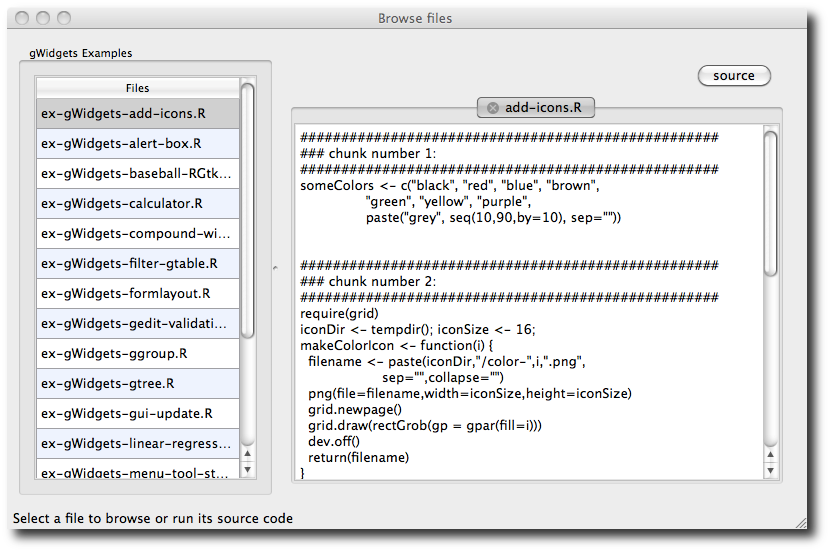
\includegraphics[width=.7\textwidth]{fig-gWidgets-example-browser}
  \caption{The example browser for gWidgets showing different layout components.}
  \label{fig:gWidgets-sample-layout}
\end{figure}



\section{Box containers}
\label{sec:gWidgets-box-containers}

The container produced by \constructor{gwindow} is intended to contain
just a single child widget, not several. This section demonstrates
variations on box containers that can be used to hold multiple child
components. Through nesting, fairly complicated layouts can be
produced.



\begin{table}
\centering
\label{tab:gWidgets-container-methods}
\caption{Container methods}
\begin{tabular}{@{}lp{0.6\textwidth}@{}}
\toprule

Method&Description\\
\midrule
\meth{add}&Adds a child object to a parent container. Called when a parent container is specified to the \args{container} argument of the widget constructor, in which case, the \args{...} arguments are passed to this method.\\\meth{delete}&Remove a child object from a parent container
\\ \bottomrule
\end{tabular}
\end{table}


\subsection{The \code{ggroup} container}
\label{sec:gWidgets-ggroup-container}
  
The basic box container is produced by \constructor{ggroup}. Its main
argument is \argument{horizontal}{ggroup} to specify whether the child
widgets are packed in horizontally from left to right (the default) or
vertically from top to bottom. 

For example, to pack a \code{cancel} and \code{ok} button into a box container we might have:
\begin{Schunk}
\begin{Sinput}
 w <- gwindow("Some buttons", visible=FALSE)
 g <- ggroup(horizontal=TRUE, cont=w)
 cancel <- gbutton("cancel", cont=g)
 ok <- gbutton("ok", cont=g)
 visible(w) <- TRUE
\end{Sinput}
\end{Schunk}

\paragraph{The add method}
When packing in child widgets, the \method{add}{ggroup} method is
used. In our example above, this is called by the
\code{gbutton} constructor when the \args{container} argument is
specified. Unlike with the underlying graphical toolkits, there is no
means to specify other styles of packing such as from the ends, or in
the middle by some index.

The \meth{add} method for box containers has a few arguments to
customize how the child widgets respond when their parent window is
resized. These are passed through the 
\args{...}  argument of the constructor.

These arguments are:
\begin{description}
\item[expand] When \code{expand=TRUE} is specified then the child
  widget will expand to fill the space allocated to it. The
  \args{fill} argument can be specified as \qcode{x}, \qcode{y}, or
  the default \qcode{both} to indicate which direction to fill
  in. 
  
  Filling varies from toolkit to toolkit, in particular
  in \pkg{gWidgetsRGtk2} one can really only specify \code{fill="both"}.
  
\item[anchor] If a widget does not expand or if it does but does not fill in both
  directions, it can be anchored into its available space in more than
  one position. The \args{anchor} argument can be specified to suggest
  where to anchor the child. It takes a numeric vector representing
  Cartesian coordinates (length two),
  with either value being \code{-1}, \code{0}, or \code{1}. For
  example, a value of \code{c(1,1)} would specify the northwest corner.
\end{description}

Figure~\ref{fig:gWidgets-ggroup-expand-fill-anchor} shows combinations
of these arguments under \pkg{gWidgetsQt}.


\begin{figure}
  \centering
  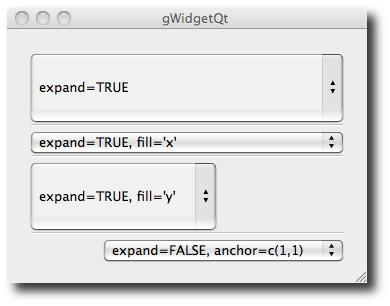
\includegraphics[width=.5\textwidth]{fig-gWidgets-ggroup-expand-fill-anchor}
  \caption{Different combinations of \code{expand}, \code{fill} and
    \code{anchor} for comboboxes in \pkg{gWidgetsQt}. The \code{fill}
    and \code{anchor} arguments
    may be overridden by the underlying toolkit for some widgets.}
  \label{fig:gWidgets-ggroup-expand-fill-anchor}
\end{figure}


\paragraph{delete}
The \method{delete}{ggroup} method can be used to remove a child
component from a container. In some toolkits, this child may be
added back at a later time, but this isn't part of the API. In the
case where you wish to hide a child temporarily, the
\meth{visible\ASSIGN} method may be used.





\paragraph{Spacing}
For spacing between the child components, the argument
\argument{spacing}{ggroup} may be used to specify, in pixels, the
amount of space between the child widgets. For \code{ggroup}
instances, this can later be set through the \method{svalue}{ggroup}
method. The method \method{addSpace}{ggroup} can add a non-uniform
amount of space between two widgets packed next to each other, whereas
the method \method{addSpring}{ggroup} will place an invisible spring
between two widgets, forcing them apart.  Both are useful for laying
out buttons.


For example, we might modify our button layout example to include a
``help'' button on the far left and the others on the right with a
fixed amount of space between them as follows:
\begin{Schunk}
\begin{Sinput}
 w <- gwindow("Some buttons", visible=FALSE)
 g <- ggroup(horizontal=TRUE, cont=w)
 help <- gbutton("help", cont=g)
 addSpring(g)
 cancel <- gbutton("cancel", cont=g)
 addSpace(g, 12)
 ok <- gbutton("ok", cont=g)
 visible(w) <- TRUE
\end{Sinput}
\end{Schunk}


To illustrate how the right panel of
Figure~\ref{fig:gWidgets-sample-layout} was done, we used nested
layouts as follows:


\begin{Schunk}
\begin{Sinput}
 g <- ggroup(horizontal=FALSE, cont=w)
 bg <- ggroup(cont=g)                    # nested group
 addSpring(bg)
 b <- gbutton("Source", cont=bg)
 nb <- gnotebook(cont=g, expand=TRUE)    # fill space
\end{Sinput}
\end{Schunk}


\paragraph{Sizing}
The overall size of a \code{ggroup} container is controlled through it
being a child of its parent container. However, a size can be assigned
through the \method{size\ASSIGN}{ggroup} method. This will be a
preferred size, but need not be the actual size, as the container may
need to be drawn larger to accomodate its children. 


For \pkg{gWidgetsRGtk2} the argument
\argument{use.scrollwindow}{ggroup}, when specified as \code{TRUE}, will
add scrollbars to the box container so that a fixed size can be
maintained. (Although, it is generally considered a poor idea to use
scrollbars when there is a chance the key controls for a dialog will
be hidden, this can be useful for displaying lists of data.)


\begin{example}{The \args{use.scrollwindow} argument}{ex-gWidgets-ggroup-use.scrollwindow}
This example shows the \args{use.scrollwindow} feature for
\pkg{gWidgetsRGtk2}. The feature is not well implemented in the other
toolkit packages. Widgets that list similar types of data are a common
part of GUIs for smart phones, say. The \function{addItem} function is used to generate
a consistent item type, in this case just a label and cancel
button. The latter shows the \method{delete}{ggroup} method for containers.

\begin{Schunk}
\begin{Sinput}
 w <- gwindow("Scroll window example", visible=FALSE)
 g <- ggroup(cont=w, horizontal=FALSE, use.scrollwindow=TRUE)
 addItem <- function(container, i) {
   g1 <- ggroup(cont=container)
   glabel(sprintf("data about %s", i), cont=g1)
   addSpring(g1)
   gimage("cancel", dir="stock", cont=g1, handler=function(h,...) {
     delete(g, g1)
   })
 }
 for(i in state.name) addItem(g, i)
 visible(w) <- TRUE
\end{Sinput}
\end{Schunk}
\end{example}

% The next example shows an alternative to the expand group widget.

% \begin{example}{The \meth{delete} method of \code{ggroup}}{ex-gWidgets-ggroup-delete}
%   \SweaveInput{ex-gWidgets-alert-box}
% \end{example}


\subsection{The \code{gframe} and \code{gexpandgroup} containers}
\label{sec:gWidgets-decorated-cont}

We discuss briefly two widgets that essentially subclass the
\code{ggroup} class. Much of the previous discussion applies.

Framed containers are used to set off its child elements using a
border and label. The \constructor{gframe} constructor produces
them. The first argument \argument{text}{gframe} is used to specify
the label. This can later be adjusted through the
\method{names\ASSIGN}{gframe} method. The argument
\argument{pos}{gframe} can be specified to adjust the label's
positioning with $0$ being the left and $1$ the right.

Although not a container, the \constructor{gseparator} widget can be
used to place a horizontal or vertical line (with the
\code{horizontal=FALSE} argument) in a layout to separate off parts of
the GUI. 


Expandable containers are useful when their child items need not be
visible all the time. The typical design involves a trigger indicator
with accompanying label indicating to the user that a click can
disclose or hide some additional information. This class subclasses
\code{gframe} where the \method{visible\ASSIGN}{gexpandgroup} method
is overridden to initiate the hiding or showing of its child area, not
the entire container.

In addition, a handler can be added that is called whenever the widget
toggles its state.


The basic framed container is used along these lines:
\begin{Schunk}
\begin{Sinput}
 w <- gwindow("gframe example")
 f <- gframe("Select a variable:", cont=w)
 vars <- gtable(names(mtcars), cont=f, expand=TRUE)
\end{Sinput}
\end{Schunk}


The usage of an expanding group is similar. Here we show how one might
leave optional the display of a statistical summary of a model.
\begin{Schunk}
\begin{Sinput}
 res <- lm(mpg ~ wt, mtcars)
 out <- capture.output(summary(res))
 w <- gwindow("gexpandgroup example")
 eg <- gexpandgroup("Summary", cont=w)
 l <- glabel(paste(out, collapse="\n"), cont=eg)
 visible(eg) <- TRUE                     # display summary
\end{Sinput}
\end{Schunk}





% \begin{example}{The \constructor{gframe} and \constructor{gexpandgroup} containers}{gWidgets-gframe-gexpandgroup-ex}
% \SweaveInput{ex-gWidgets-gframe-gexpandgroup.Rnw}
% \end{example}




\section{Paned containers: the \code{gpandedgroup} container}
\label{sec:gWidgets-gpanedgroup-container}

The \constructor{gpanedgroup} constructor produces a container which
has two children which are separated by a visual gutter which can be
adjusted by the user with their mouse to allocate the space between the two
children. Figure~\ref{fig:gWidgets-sample-layout} uses such a
container to separate the file selection controls from the file
display ones.  For this container, the children are aligned
side-by-side (by default) or top to bottom if the
\argument{horizontal}{gpanedgroup} argument is given as
\code{FALSE}. 


To add children, the container should be used as the parent container
for two constructors. These can be other container constructors which
is the typical usage for more complicated layouts.
(For toolkits which support the separation of widget
construction and layout, the \constructor{gpanedgroup} constructor can
have two children specified to the arguments
\argument{widget1}{gpanedgroup} and \argument{widget2}{gpanedgroup}.)

The main property of this container is the sash position, a value in
$[0,1]$. This may be configured programatically
through the \method{svalue\ASSIGN}{gpanedgroup} method, where a value
from 0 to 1 specifies the proportion of space allocated to the
leftmost (topmost) child. This specification only works after the
containing window is drawn, as the percentage is based on the size of
the window.


A simplified version of the layout in
Figure~\ref{fig:gWidgets-sample-layout} would be
\begin{Schunk}
\begin{Sinput}
 d <- system.file("Examples/ch-gWidgets", package="ProgGUIinR")
 files <- list.files(d)
 w <- gwindow("gpanedgroup example", visible=FALSE)
 pg <- gpanedgroup(cont = w)
 tbl <- gtable(files, cont=pg)
 t <- gtext("", cont=pg, expand=TRUE)
 visible(w) <- TRUE
 svalue(pg) <- 0.33                      # after drawing
\end{Sinput}
\end{Schunk}


% \begin{example}{Paned groups}{ex-gWidgets-panedgroups}
%   This example shows how one could use this container.
% <<keep.source=TRUE>>=
% w <- gwindow("gpanedgroup example", visible=FALSE)
% pg <- gpanedgroup(cont=w)
% g <- ggroup(cont=pg)                  # left child
% l <- glabel("left child", cont=g)
% b <- gbutton("right child", cont=pg)
% visible(w) <- TRUE
% @ 
% To adjust the sash position, one can do:
% <<>>=
% svalue(pg) <- 0.75
% @ 
% \end{example}


  
\section{Tabbed notebooks: the \code{gnotebook} container}
\label{sec:gWidgets-gnotebook}

The \constructor{gnotebook} constructor produces a tabbed notebook
container. The GUI in Figure~\ref{fig:gWidgets-sample-layout} uses a
notebook to hold different text widgets, one for each file being displayed.

The \pkg{gWidgets}constructor has a few arguments. The argument
\argument{tab.pos}{gnotebook} is used to specify the location of the
tabs using a value of 1 through 4 with 1 being botton, 2 left side, 3
top and 4 right side being used, with the default being 3 (similar
numbering is used in \function{par}). The
\argument{closebuttons}{gnotebook} argument takes a logical indicating
whether the tabs should have close buttons on them. In this case, the
argument \argument{dontCloseThese}{gnotebook} can be used to specify
which tabs, by index, should not be closable. (As of writing, this is
not implemented in  \pkg{gWidgetstcltk}.)



\paragraph{Methods}
Pages are added through the \method{add}{gnotebook} method for the
notebook container. The extra a \argument{label}{add} argument is used
to specify the tab label. (As \meth{add} is called implicitly when a a
widget is constructed, this argument is usually specified to the
constructor.)



The \method{svalue}{gnotebook} method returns the index of the
currently raised tab, whereas \method{svalue\ASSIGN}{gnotebook} can be
used to switch the page to the specified tab. The currently shown tab
can be removed using the \method{dispose}{gnotebook} method. To remove
a different tab, use this method in combination with
\meth{svalue\ASSIGN}. (When removing many tabs, you will want to start
from the end as otherwise the tab positions change during removal.)

From some viewpoint, the notebook widget is viewed as a vector with a
names attribute (the labels) and components being the child
components. As such, the \method{names}{gnotebook} method can be used
to retrieve the tab names, and \method{names\ASSIGN}{gnotebook} to set
the names. The \method{length}{gnotebook} method returns the number of
pages held by the notebook. The \meth{[} is also implemented to return the
child components.



\begin{example}{Tabbed notebook example}{ex-gWidgets-gnotebook}
 In theh GUI of Figure~\ref{fig:gWidgets-sample-layout} a notebook is
 used to hold differing pages. The following is the basic setup used.
\begin{Schunk}
\begin{Sinput}
 w <- gwindow("gnotebook example")
 nb <- gnotebook(cont=w)
\end{Sinput}
\end{Schunk}

New pages are added as follows:
\begin{Schunk}
\begin{Sinput}
 fname <- "DESCRIPTION"                  # or something else
 f <- system.file(fname, package="gWidgets")
 gtext(readLines(f), cont = nb, label=fname)
\end{Sinput}
\begin{Soutput}
guiWidget of type: gTextRGtk for toolkit: guiWidgetsToolkitRGtk2 
\end{Soutput}
\end{Schunk}

To manipulate the displayed pages, say to set the page to the last one
we have:
\begin{Schunk}
\begin{Sinput}
 svalue(nb) <- length(nb)
\end{Sinput}
\end{Schunk}
To remove the current  page
\begin{Schunk}
\begin{Sinput}
 dispose(nb)
\end{Sinput}
\end{Schunk}
%
\end{example}

\section{Grid layout: the \code{glayout} container}
\label{sec:gWidgets-glayout-container}

The layout of dialogs and forms is usually seen with some form of
alignment between the widgets. The \constructor{glayout} constructor
provides a grid container to do so, using matrix notation to specify
location of the children.  

To see its use, we can layout a simple form for collecting information
as follows:

\begin{Schunk}
\begin{Sinput}
 w <- gwindow("glayout example", visible=FALSE)
 tbl <- glayout(cont=w, spacing=5)
 right <- c(1,0); left <- c(-1,0)
 tbl[1,1, anchor=right] <- "name"
 tbl[1,2, anchor=left ] <- (name <- gedit("", cont=tbl))
 tbl[2,1, anchor=right] <- "rank"
 tbl[2,2, anchor=left ] <- (rank <- gedit("", cont=tbl))
 tbl[3,1, anchor=right] <- "serial number"
 tbl[3,2, anchor=left ] <- (snumber <- gedit("", cont=tbl))
 visible(w) <- TRUE
\end{Sinput}
\end{Schunk}


The constructor has a few arguments to configure the appearance of the
container. The spacing between each cell may be specified through the
\argument{spacing}{glayout} argument, the default is 10 pixels. A
value of 5 is used above to tighten up the display.
To impose a uniform cell size, the \argument{homogeneous}{glayout}
argument can be specified with a value of \code{TRUE}. The default is
\code{FALSE}. 

As seen, children may be added to the grid at a specific row and
column. To specify this, \R's matrix notation, \code{[\ASSIGN}, is
used with the indices indicating the row and column.  A child may span
more than one row or column. The corresponding index should be a
vector of indices indicating so.  The \code{[} method may be used to
return the child occupying position $i,j$.


To add a child, the \code{glayout} container should be specfied as the
\code{container} and be on the left hand side of the \code{[\ASSIGN}
call. (This is necessary only for the toolkits where a container must
be specified, where the right hand side is used to pass along the
parent information and the left hand side is used for the layout.) For
convenience, if the right hand side is a string, a label will be
generated.  To align a widget within a cell, the
\argument{anchor}{add} argument of the \code{[\ASSIGN}{glayout} method
is used. The example above illustrates how this can be used to achieve
a center balance.


% \begin{example}{Layout with \constructor{glayout}}{ex-gWidgets-glayout}
%   This example shows how a simple form can be given an center-balanced
%   layout using a grid container. 

% \end{example}







\chapter{\pkg{gWidgets}: Control Widgets}
\label{cha:control-widgets}
%% orgainze by function

\XXX{Where to integrate methods such as enabled?}
\XXX{stock icons}
\XXX{addHandler text -- done here with first, but could be elsewhere}
\XXX{drag and drop example}
  

  
This section discusses the basic controls provided by
\pkg{gWidgets}.

\begin{table}
\centering
\label{tab:gWidgets-control-widgets}
\caption{Table of constructors for control widgets in \pkg{gWidgets}. Most, but not all, are implemented for each toolkit.}
\begin{tabular}{@{}lp{0.7\textwidth}@{}}
\toprule

Constructor&Description\\
\midrule
\constructor{glabel}&A text label\\\constructor{gbutton}&A button to initiate an action \\\constructor{gcheckbox}&A checkbox\\\constructor{gcheckboxgroup}&A group of checkboxes\\\constructor{gradio}&A radio button group\\\constructor{gcombobox}&A drop-down list of values, possible editable\\\constructor{gtable}&A table (vector or data frame) of values for selection\\\constructor{gslider}&A slider to select from a sequence value\\\constructor{gspinbutton}&A spinbutton to select from a sequence of values\\\constructor{gedit}&Single line of editable text\\\constructor{gtext}&Multi-line text edit area\\\constructor{ghtml}&Display text marked up with HTML\\\constructor{gdf}&Data frame viewer and editor\\\constructor{gtree}&A display for heirarchical data\\\constructor{gimage}&A display for icons and images\\\constructor{ggraphics}&A widget containing a graphics device\\\constructor{gsvg}&A widget to display SVG files\\\constructor{gfilebrowser}&A widget to select a file or directory\\\constructor{gcalendar}&A widget to select a date\\\constructor{gaction}&A resusable definition of an action\\\constructor{gmenubar}&Adds a menubar on a top-level window \\\constructor{gtoolbar}&Adds a toolbar to a top-level window\\\constructor{gstatusbar}&Adds a status bar to a top-level window\\\constructor{gtooltip}&Add a tooltip to widget\\\constructor{gseparator}&A widget to display a horizontal or vertical line
\\ \bottomrule
\end{tabular}
\end{table}%% place these as approporiate
% \begin{table}
%   \centering
%   \begin{tabular}{l@{\quad}p{.75\textwidth}}
% %    \toprule
%     \constructor{glabel} & A text label\\
%     \constructor{gbutton} & A button to initiate an action \\
%     \constructor{gcheckbox} & A checkbox widget\\
%     \constructor{gradio} & Constructs a radio button group\\
%     \constructor{gcheckboxgroup} & Constructs a group of checkboxes\\
%     \constructor{gcombobox} & Constructs drop down list of values\\
%     \constructor{gtable} & Shows a table (vector or data frame) of
%     values for selection\\ 
%     \constructor{gslider} & A slider to select a value\\
%     \constructor{gspinbutton} & A spinbutton to select from a set of values\\
%     \constructor{gedit} & One line of editable text\\
%     \constructor{gtext} & multi-line text edit\\
%     \constructor{ghtml} & Display text marked up with HTML\\
%     \constructor{gdf} & Data frame viewer and editor\\
%     \constructor{gtree} & Displays heirarchical data\\
%     \constructor{gimage} & Displays icons and images\\
%     \constructor{ggraphics} & A widget containing a graphics device\\
%     \constructor{gfilebrowser} & A widget to select a file or directory\\
%     \constructor{gcalendar} & A widget to select a date\\
%     \constructor{gaction} & a resusable definition of an action\\
%     \constructor{gmenubar} & Puts a menubar on a top-level window\\    
%     \constructor{gtoolbar} & Adds a toolbar to a top-level window\\
%     \constructor{gstatusbar} & Adds a status bar to a top-level window\\
%     \constructor{gseparator} & A widget to display a horizontal or vertical line\\
%     \bottomrule
%   \end{tabular}
%   \caption{Table of basic control constructors in \pkg{gWidgets}}
%   \label{tab:gWidgets-control-widgets}  
% \end{table}


\subsection{Buttons}
\label{sec:gWidgets-buttons}

The button widget allows a user to initiate an action through clicking
on it. Buttons have labels, conventionally verbs indicating action,
and often icons. The \constructor{gbutton} constructor has an argument
\argument{text}{gbutton} to specify the text.  For text that matches
the stock icons of \pkg{gWidgets}
(Section~\ref{sec:gWidgets-displ-icons-imag}) an icon will
appear. (The \code{ok} button below, but not the custom \code{par...} one.)

In common with the other controls, the argument
\argument{handler}{gbutton} is used to specify a callback and the
\argument{action}{gbutton} argument will be passed along to this
callback (unless it is a \code{gaction} object, whose case is described
in Section~\ref{sec:gWidgets-actions}).
The default handler is the click handler which can be specified at
construction, or afterward through 
\method{addHandlerClicked}{gbutton}.

The following example shows how a button can be used to call a sub
dialog to collect optional information. We imagine this as part of a
dialog to generate a plot.

\begin{Schunk}
\begin{Sinput}
 w <- gwindow("Make a plot")
 g <- ggroup(horizontal=FALSE, cont=w)
 glabel("... Fill me in ...", cont=g)
 bg <- ggroup(cont=g)
 addSpring(bg)
 parButton <- gbutton("par...", cont=bg)
 addHandlerClicked(parButton, handler=function(h,...) {
   w1 <- gwindow("Set par values...", parent=w)
   lyt <- glayout(cont=w1)
   lyt[1,1, align=c(-1,0)] <- "mfrow: c(nr,nc)"
   lyt[2,1] <- (nr <- gedit(1, cont=lyt))
   lyt[2,2] <- (nc <- gedit(1, cont=lyt))
   lyt[3,2] <- gbutton("ok", cont=lyt, handler=
                       function(h,...) {
                         x <- as.numeric(c(svalue(nr), svalue(nc)))
                         par(mfrow=x)
                         dispose(w1)
                       })
 })
\end{Sinput}
\end{Schunk}



%% methods
The button's label is its main property and can be queried or set with
The \method{svalue}{gbutton} or \method{svalue\ASSIGN}{gbutton}.  Most
GUIs will make a button insensitive to user input if the button's
action is not currently permissible. Toolkits draw such buttons in a
grayed-out state. As with other components, the \method{enabled\ASSIGN}{gWidgets} method can set
or disable whether a widget can accept input.

%% Default
% A new button may or may not have the focus when a GUI is
% constructed. If it does have the focus, then the \kbd{return} key will
% initiate the button click signal. To make a GUI start with its focus
% on a button, the \method{defaultWidget}{gWidgets} method is available. 


% A basic example of a button with a handler was given in Example~\ref{ex-gWidgets-hello-world-button}.

%% ML: I don't think it would hurt to see something like that
%% again. The reader will expect an example here.

% As an example of the limitations of \pkg{gWidgets} compared to the
% underlying toolkits, within \pkg{gWidgets} there are no methods to set
% an icon, or add an mnemonic to the button.


% \begin{example}{Hello world button}{ex-gWidgets-hello-world-button}
%   This example shows how a button is assigned a handler to respond to
%   click events.~\footnote{Each toolkit has its idiosyncracies. If this
%     example is run using \pkg{RGtk2} the button will stretch to fill
%     the space. At times this is not desired. Placing the button within
%     a \code{ggroup} container can prevent this. Whereas, under
%     \code{tcltk} the parent window will shrink to fit the button. The
%     \meth{size} method can prevent this if it is not desired.} When
%   working with handlers, one can use an object name that will be found
%   through \R's scoping rules, or the components passed through the
%   \code{h} argument, as below.

% <<>>=
% w <- gwindow("Button example")
% b <- gbutton("Click me", cont=w)
% id <- addHandlerChanged(b, action=w, handler=function(h,...) {
%   btnText <- svalue(h$obj)                   # or svalue(b)
%   svalue(h$obj) <- paste("don't", btnText, "again") # set text
%   enabled(h$obj) <- FALSE
%   svalue(h$action) <- "Button example is finished" # set title
% })

% @ 

% \end{example}


\subsection{Labels}
\label{asec:gWidgets-labels}

The \constructor{glabel} constructor produces a basic label
widget. We've seen its use in a number of examples. The main property,
the label's text, is specified through the \argument{text}{glabel}
argument. This is a character vector of length 1 or is coerced into
one by collapsing the vector with newlines. The
\method{svalue}{glabel} method will return the label text as a single
string, whereas the \method{svalue\ASSIGN}{glabel} method is avaialable
to set the text programatically.

The \method{font\ASSIGN}{glabel} method
can also be used to set the text markup
(Table~\ref{tab:gWidgets-font-properties}).  For \pkg{gWidgetsRGtk2} the
argument \argument{markup}{glabel} for the constructor takes a logical
value indicating if the text is in the native markup language (PANGO).


For example, to make a form's labels have some emphasis we could do:
\begin{Schunk}
\begin{Sinput}
 w <- gwindow("label example")
 f <- gframe("Summary statistics:", cont=w)
 lyt <- glayout(cont=f)
 lyt[1,1] <- glabel("xbar:", cont=lyt)
 lyt[1,2] <- gedit("", cont=lyt)
 lyt[2,1] <- glabel("s:", cont=lyt)
 lyt[2,2] <- gedit("", cont=lyt)
 sapply(1:2, function(i) {
   tmp <- lyt[i,1]
   font(tmp) <- c(weight="bold", color="blue")
 })
\end{Sinput}
\end{Schunk}


The widget constructor also has the argument
\argument{editable}{glabel}, which when specified as \code{TRUE} will
add a handler to the event so that the text can be edited when the
label is clicked.  Although this is popular in some familiar
interfaces, such as a spreadsheet tab, it has not proven to be
intuitive to most users, as labels are not generally expected to change.


\subsection{Statusbars}
\label{sec:gWidgets-statusbars}

Statusbars are simply labels placed at the bottom of a top-level window to leave
informative, but non-disruptive, messages for the user.  The
\constructor{gstatusbar} constructor provides this widget.  The
\args{container} argument should be a top-level window instance. 
The only property is the label's text. This may be specified at
construction with the argument
\argument{text}{gstatusbar}. Subsequent changes are made through
the \method{svalue\ASSIGN}{gstatusbar} method. 




\subsection{Displaying icons and images stored in files}
\label{sec:gWidgets-displ-icons-imag}

The \pkg{gWidgets} package provides a few stock icons that can be
added to various GUI components. A list of the defined stock icons is
returned by the function \code{getStockIcons}.  The names attribute
defines the valid stock icon names. It was mentioned that if a
button's label matches a stock icon name, that icon will appear
adjacent to the label.



%% gimage
Other graphic files and the stock icons can be displayed by the
\constructor{gimage} widget. \footnote{Not all file types may be
  displayed by each toolkit, in particular \pkg{gWidgetstcltk} can
  only display gif, ppm, and xbm files.} The file to display is
specified through the \argument{filename}{gimage} argument of the
constructor. This value is combined with that of the
\argument{dirname}{gimage} argument to specify the file path.  Stock
icons, can be specified by using their name for the \code{filename}
argument and the character string \code{"stock"} for the
\code{dirname} argument.~\footnote{For \pkg{gWidgetsRGtk2}, the size
  of a stock icon can be adjusted through the \argument{size}{gimage}
  argument, with a value from \qcode{menu}, \qcode{small\_toolbar},
  \qcode{large\_toolbar}, \qcode{button}, or \qcode{dialog}.}
%% methods

The \method{svalue\ASSIGN}{gimage} method is used to change the
displayed file. In this case, a full path name is specified, or the
stock icon name.

The default handler is a button click handler.


To illustrate, a simple means to display a graphic (except in
\pkg{gWidgetstcltk} where png support is not available) is
as follows:
\begin{Schunk}
\begin{Sinput}
 f <- tempfile()
 png(f)
 hist(rnorm(100))
 dev.off()
 w <- gwindow("Example to show a graphic")
 gimage(basename(f), dirname(f), cont=w)
\end{Sinput}
\end{Schunk}


More stock icon names may be added through the function
\code{addStockIcons}. This function requires a vector of stock icon
names and a vector of corresponding file paths, and is illustrated
through an example.


\begin{example}{Adding and using stock icons}{ex-gWidgets-stock-icons}
This example shows how to add to the available stock icons and use
\code{gimage} to display them. It creates a table to select a color
from, as an alternative to a more complicated color chooser
dialog. Under \pkg{gWidgetstcltk} the image files would need to be
converted to \code{gif} format, as \code{png} format is not a natively
supported image type.

We begin by defining 16 arbitrary colors.

\begin{Schunk}
\begin{Sinput}
 someColors <- c("black", "red", "blue", "brown",
                 "green", "yellow", "purple",
                 paste("grey", seq(10,90,by=10), sep=""))
\end{Sinput}
\end{Schunk}

This is the function that is used to create an icon file. We use some
low-level \pkg{grid} functions to draw the image to a png file.
\begin{Schunk}
\begin{Sinput}
 require(grid)
 iconDir <- tempdir(); iconSize <- 16;
 makeColorIcon <- function(i) {
   filename <- paste(iconDir, "/color-", i, ".png",
                     sep="", collapse="")
   png(file=filename, width=iconSize, height=iconSize)
   grid.newpage()
   grid.draw(rectGrob(gp=gpar(fill=i)))
   dev.off()
   return(filename)
 }
\end{Sinput}
\end{Schunk}

To add icons, we need to define the stock names and the file paths for
\code{addStockIcons}.

\begin{Schunk}
\begin{Sinput}
 icons <- sapply(someColors, makeColorIcon)
 iconNames <- paste("color-", someColors, sep="")
 addStockIcons(iconNames, icons)
\end{Sinput}
\end{Schunk}

We use a table layout to show the 16 colors. As an illustration of
assigning a handler for a click event, we assign one that returns the
corresponding stock icon name.

\begin{Schunk}
\begin{Sinput}
 w <- gwindow("Icon example")
 f <- function(h,...) print(h$action)
 tbl <- glayout(cont=w, spacing=0)
 for(i in 1:4) {
   for(j in 1:4) {
     ind <- (i - 1) * 4 + j
     tbl[i,j] <- gimage(icons[ind], handler=f, 
                        action=iconNames[ind], cont=tbl)
   }
 }
\end{Sinput}
\end{Schunk}
\end{example}

Finally, we mention the \constructor{gsvg} constructor is similar to \constructor{gimage}, but allows one to
display SVG files, as produced by the \function{svg} driver, say. It
currently is only available for \pkg{gWidgetsQt}.

\section{Text editing controls}
\label{sec:gWidgets-text-edit-contr}



\subsection{Single-line, editable text}
\label{sec:gWidgets-single-line-editable}

The \pkg{gWidgets} package, following the underlying toolkits, has two
main widgets for editing text: \constructor{gedit} for a single line
of editable text, and \constructor{gtext} for multi-line, editable
text.  For some toolkits, a \constructor{ghtml} widget is also
defined, but neither \pkg{gWidgetsRGtk2} nor \pkg{gWidgetstcltk} have this
implemented.


The \constructor{gedit} constructor produces a widget to display a
single line of editable text. The main property is the initial text
which can be set through the \argument{text}{gedit} argument.  If it
is desirable to set the width of the widget, the
\argument{width}{gedit} argument allows the specification in terms of
number of characters allowed to display without horizontal
scrolling. The width of the widget may also be specified in pixel size
through the \method{size}{guiWidget} method.


\paragraph{Methods}
The text is returned by the \method{svalue}{gedit} method and may be
set through the \method{svalue\ASSIGN}{gedit} method.  The
\meth{svalue} method will return a character vector by
default. However, it may be desirable to use this widget to collect
numeric values or perhaps some other type of variable. One could write
code to coerce the character to the desired type, but it is sometimes
convenient to have the return value be a certain non-character
type. In this case, the \argument{coerce.with}{gedit} argument can be
used to specify a function of a single argument to call before the
value is returned by \meth{svalue}.

Some toolkits allow type-ahead values to be set. These values
anticipate what a user wishes to type and offers a means to complete a
word. The \method{[\ASSIGN}{gedit} method allows these values to be
specifed through a character vector, as in \code{obj[] \ASSIGN\/ values}.

For example, the following can be used to collect one of the 50 state
names in the U.S.:
\begin{Schunk}
\begin{Sinput}
 w <- gwindow("gedit example") 
 g <- ggroup(cont=w)
 glabel("State name:", cont=g)
 e <- gedit("", cont=g)
 e[] <- state.name
\end{Sinput}
\end{Schunk}

\paragraph{Handlers}
The default handler for the \constructor{gedit} widget is called when
the text area is ``activated'' through the
\kbd{return} key being pressed. Use \meth{addHandlerBlur} to add a
callback for the event of losing focus. The
\method{addHandlerKeystroke}{gedit} method can assign a handler to be
called when a key is released. For the toolkits that support it, the
specific key is given in the \code{key} component of the list \code{h} (the first component).

\begin{example}{Validation}{ex-gWidgets-gedit-validation}
GUIs for \R\/ may differ a bit from many GUIs one typically interacts
with, as \R\/ users expect to be able to use variables and expressions
where typically one uses just characters or numbers. As such, one
needs to evaluate expressions. This example shows how to implement a
validation framework on a single-line edit widget so that the user has
feedback if an expression will not evaluate properly.  If the value is
invalid, we set the text color to red. 


We use a table to layout out example:
\begin{Schunk}
\begin{Sinput}
 w <- gwindow("Validation example")
 tbl <- glayout(cont=w)
 tbl[1,1] <- "R expression:"
 tbl[1,2] <- (e <- gedit("", cont = tbl))
\end{Sinput}
\end{Schunk}


We use the \pkg{evaluate} package to see if the expresssion is valid.
\begin{Schunk}
\begin{Sinput}
 require(evaluate)
 isValid <- function(e) {
   out <- try(evaluate:::evaluate(e), silent=TRUE)
   !(inherits(out, "try-error") || 
     is(out[[2]], "error"))
 }
\end{Sinput}
\end{Schunk}
%

We validate our expression when the user commits the change, by
pressing the return key while the widget has focus. Alternatively, we
could have used
\code{addHandlerKeystroke}, to validate after each key press, or
\code{addHandlerBlu}, to validate when the widget loses focus.

\begin{Schunk}
\begin{Sinput}
 addHandlerChanged(e, handler = function(h,...) {
   curVal <- svalue(h$obj)
   if(isValid(curVal)) {
     font(h$obj) <- c(color="black")
   } else {
     font(h$obj) <- c(color="red")
     focus(h$obj) <- TRUE
   }
 })
\end{Sinput}
\end{Schunk}

\end{example}

\subsection{Multi-line, editable text}
\label{sec:gWidgets-multi-line-editable}

The \constructor{gtext} constructor produces a multi-line text editing
widget with scrollbars to accommodate large amounts of text. The
\argument{text}{gtext} argument is for specifying the intial
text. The initial width and height can be
set through similarly named arguments, which is useful with
\pkg{gWidgetstcltk}. 

The \method{svalue}{gtext} method retrieves the text stored in the
buffer. If the argument \code{drop=TRUE} is specified, then only the
currently selected text will be returned. Text in multiple lines is
returned as a single string with ``\backslashn'' separating the lines.

The contents of the text buffer can be replaced with the
\method{svalue\ASSIGN}{gtext} method. To clear the buffer, the
\method{dispose}{gtext} method can be used. The \method{insert}{gtext}
method adds text to a buffer. The signature is \code{insert(obj, text,
  where, font.attr)}
where \code{text} is a character vector. New text is added to the end
of the buffer, by default, but the \argument{where}{insert} argument
can specify \qcode{beginning} or \qcode{at.cursor}.




As with \code{gedit}, the \method{addHandlerKeystroke}{gtext} method
sets a handler to be called for each keystroke. This is the default
handler.

\paragraph{fonts}
Fonts can be specified for the entire buffer or the selection using
the specifications in Table~\ref{tab:gWidgets-font-properties}. To
specify fonts for the entire buffer use the
\argument{font.attr}{gtable} argument of the constructor. The
\method{font\ASSIGN}{gtext} method serves the same purpose, provided
there is no selection when called. If there is a selection, the font
change will only be applied to the selection. Finally, the
\argument{font.attr}{insert} argument for the \meth{insert} method
specifies the font attributes for the inserted text.

\begin{table}
\centering
\label{tab:gWidgets-font-properties}
\caption{Possible specfications for setting font properties. Font values of an object are changed with named vectors, as in \code{font(obj)\ASSIGN c(weight="bold", size=12, color="red")}}
\begin{tabular}{@{}lp{0.6\textwidth}@{}}
\toprule

Attribute&Possible value\\
\midrule
weight&light, normal, bold\\style&normal, oblique, italic\\family&normal, sans, serif, monospace\\size&a point size, such as 12\\color&a named color
\\ \bottomrule
\end{tabular}
\end{table}
\begin{example}{A calculator}{ex-gWidgets-calculator}
%% A calculator layout example
The following example shows how one might use the widgets just
discussed to make a GUI that resembles a calculator. Such a GUI may offer
familiarity to new \R\/ users, although certainly is no replacement
for a command line.

The \constructor{glayout} container is used to neatly arrange the
widgets. This example illustrates how a child widget can span a block
of multiple cells by using the appropriate indexing. Furthermore, the
\args{spacing} argument is used to tighten up the appearance. The
example also illustrates a useful strategy of storing the widgets
using a list for subsequent manipulations.

The following sets up the layout of the display and buttons.
\begin{Schunk}
\begin{Sinput}
 buttons <- rbind(c(7:9, "(", ")"),
                  c(4:6, "*", "/"),
                  c(1:3, "+", "-"))
 bList <- list()
 w <- gwindow("glayout for a calculator")
 g <- ggroup(cont=w, expand=TRUE, horizontal=FALSE)
 tbl <- glayout(cont=g, spacing=2)
 tbl[1, 1:5, anchor=c(-1,0)] <-          # span 5 columns
   (eqnArea <- gedit("", cont=tbl))
 tbl[2, 1:5, anchor=c(1,0)] <- 
   (outputArea <- glabel("", cont=tbl))
 for(i in 3:5) {
   for(j in 1:5) {
     val <- buttons[i-2, j]
     tbl[i,j] <- (bList[[val]] <- gbutton(val, cont=tbl))
   }
 }
 tbl[6,2] <- (bList[["0"]] <- gbutton("0", cont=tbl))
 tbl[6,3] <- (bList[["."]] <- gbutton(".", cont=tbl))
 tbl[6,4:5] <- (eqButton <- gbutton("=", cont=tbl))
 outputArea <- gtext("", cont = g)
\end{Sinput}
\end{Schunk}

This code defines the handler for each button except the equals button
and then assigns the handler to each button. This is done efficiently,
using the generic \meth{addHandlerChanged}. The handler simply pastes
the text for each button into the equation area.

\begin{Schunk}
\begin{Sinput}
 addButton <- function(h, ...) {
   curExpr <- svalue(eqnArea)
   newChar <- svalue(h$obj)              # the button's value
   svalue(eqnArea) <- paste(curExpr, newChar, sep="")
   svalue(outputLabel) <- ""             # clear label 
 }
 out <- sapply(bList, function(i) 
               addHandlerChanged(i, handler=addButton))
\end{Sinput}
\end{Schunk}

When the equals sign is clicked, the expression is evaluated and if
there are no errors, the output is displayed in the label.
\begin{Schunk}
\begin{Sinput}
 addHandlerClicked(eqButton, handler = function(h,...) {
   curExpr <- svalue(eqnArea)
   out <- try(capture.output(eval(parse(text=curExpr))), silent=TRUE)
   if(inherits(out,"try-error")) {
     galert("There is an error")
   } else {
     svalue(outputArea) <- out
     svalue(eqnArea) <- ""            # restart
   }
 })
\end{Sinput}
\end{Schunk}

\end{example}

\section{Selection controls}
\label{sec:gWidgets-widg-select-data}

A common task for a GUI control is to select a value or values from a
set of numbers or a table of numbers. Many toolkits implement these
widgets using a model-view-controller paradigm whereby the control is
just one of possibly many views of the data model. This
approach is not used by \pkg{gWidgets}. Rather, each widget has its
own data store (like a vector or data frame)
containing the data for selection, and familar \R\/ methods are used to
manipulate this underlying data store. The controls in \pkg{gWidgets} that
display such data have the methods \code{[}, \code{[\ASSIGN},
\code{length}, \code{dim}, \code{names} and \code{names\ASSIGN}, as
appropriate.

This section discusses several selection controls that serve a similar
purpose but make different use of screen space.

\subsection{Checkbox widget}
\label{sec:gWidgets-checkbox-widget}

The simplest selection control is the \constructor{checkbox} widget
that allows the user to set a state as \code{TRUE} or
\code{FALSE}. The constructor has an argument
\argument{text}{gcheckbox} to set a label and
\argument{checked}{gcheckbox} to indicate if the widget should
initially be checked. The default is \code{TRUE}. By default the label
will be drawn aside a checkbox, if the argument
\argument{use.togglebutton}{gcheckbox} is \code{TRUE}, a toggle button
-- which appears depressed when \code{TRUE} -- is used.

The \method{svalue}{gcheckbox} method returns a logical indicating if
the widget is in the checked state. Use \method{svalue\ASSIGN}{gcheckbox} to set
the state. The label's value is returned by the
\method{[}{gcheckbox} method, and can be adjusted through 
\method{[\ASSIGN}{gcheckbox}. (We take the abstract view that the user
is selecting, or not, from the length-1 vector, so \meth{[} is used to
set the data to select from.)

The default handler would be called on a click event, when the state toggles. If it is desired
that the handler be called only in the \code{TRUE} state, say, one
needs to check within the handler for this. For example

\begin{Schunk}
\begin{Sinput}
 w <- gwindow("checkbox example")
 cb <- gcheckbox("label", cont=w, handler=function(h,...) {
   if(svalue(h$obj))                     # it is checked
     print("define handler here")
 })
\end{Sinput}
\begin{Soutput}
[1] "DEBUG"
[1] FALSE
\end{Soutput}
\end{Schunk}

\subsection{Radio button widget}
\label{sec:gWidgets-radio-button-widget}

A radio button group allows the user to choose one of a few
items. A radio button group object is returned by
\constructor{gradio}. The items to choose from are specified as a
vector of values to the \argument{items}{gradio} argument (2 or more). These items
may be displayed horizontally or vertically (the default) as specified by the
\argument{horizontal}{gradio} argument which expects a logical. The
\argument{selected}{gradio} argument specifies the initially selected
item, by index,
with a default of the first.

The currently selected item is returned by \method{svalue}{gradio} as
the label text or by the index if the argument \args{index} is
\code{TRUE}. The item may be set with the
\method{svalue\ASSIGN}{gradio} method. Again, the item may be
specified by the label or by an index, the latter when the argument
\code{index=TRUE} is specified. The data store is the set of labels so
are referenced through the \method{[}{gradio} method, and may be set
(if the underlying toolkit allows it) with the
\method{[\ASSIGN}{gradio} method. (In \pkg{gWidgetstcltk} one can not
change the number of radio buttons.) For convenience, the
\method{length}{gradio} method returns the number of labels.

The handler, if given to the constructor or set with \meth{addHandlerChanged}, is called on a click event.

\subsection{A group of checkboxes}
\label{sec:gWidgets-group-checkboxes}


The checkbox group widget, produced by the
\constructor{gcheckboxgroup} constructor, is similar to a radio group,
but allows the selection of one or more of a set of items.  The
\argument{items}{gcheckboxgroup} arugment is used to specify the
values. The state of whether an item is selected can be set with a
logical vector of the same size as the number of items to the
\argument{checked}{gcheckboxgroup} argument; recycling is used. The
item layout can be controlled by the
\argument{horizontal}{gcheckboxgroup} argument. The default is a
vertical layout (\code{horizontal=FALSE}).

The state is retrieved as a character vector through the
\method{svalue}{gcheckboxgroup} method. The \code{index=TRUE} argument
instructs \meth{svalue} to return the indices instead. As a
checkboxgroup is like both a checkbox and a radio button group, one
can set the selected values two different ways. As with a checkbox, 
the selected values can be set by specifying a logical vector through the
\method{svalue\ASSIGN}{gcheckboxgroup} method. As with radio button groups,
the selected values can also be set with a character vector indicating
which labels should be selected, or if \code{index=TRUE} is given,
using a numeric index vector.

The labels are returned through the \method{[}{gcheckboxgroup} method
and if the underlying toolkit allows it, set through the
\method{[\ASSIGN}{gcheckboxgroup} method. As with \constructor{gradio},
the \method{length}{gcheckboxgroup} method returns the number of items.

As an illustration of the related selection widgets, the following
could be part of a GUI to illustrate densities for various kernels.
\begin{Schunk}
\begin{Sinput}
 kerns <- as.character(formals(density.default)$kernel)[-1]
 w <- gwindow("Arguments for density example")
 lyt <- glayout(cont=w)
 lyt[1,1] <- "bw"
 lyt[1,2, anchor=c(-1,0)] <- 
   gradio(c("nrd0", "nrd", "ucv", "bcv", "SJ"), cont=lyt)
 lyt[2,1] <- "Kernel"
 lyt[2,2, anchor=c(-1,0)] <- gcheckboxgroup(kerns, cont=lyt)
\end{Sinput}
\begin{Soutput}
[1] "DEBUG"
[1] FALSE
[1] "DEBUG"
[1] FALSE
[1] "DEBUG"
[1] FALSE
[1] "DEBUG"
[1] FALSE
[1] "DEBUG"
[1] FALSE
[1] "DEBUG"
[1] FALSE
[1] "DEBUG"
[1] FALSE
\end{Soutput}
\begin{Sinput}
 lyt[3,1] <- "na.rm"
 lyt[3,2, anchor=c(-1,0)] <- 
   gcheckbox("na.rm", checked=TRUE, use.togglebutton=TRUE, cont=lyt)
\end{Sinput}
\begin{Soutput}
[1] "DEBUG"
[1] TRUE
\end{Soutput}
\begin{Sinput}
 lyt[4,2] <- gbutton("done", cont=lyt, handler=function(h,...) {
   out <- sapply(1:3, function(i) {
     widget <- lyt[i,2]
     svalue(widget)
   })
   print(out)                            # make a plot...
 })
\end{Sinput}
\end{Schunk}

\subsection{A combobox}
\label{sec:gWidgets-combobox}

A combobox is used as an alternative to a radio button group when
there are too many choices to comfortably fit on the screen. Comboboxes are
constructed by \constructor{gcombobox}. The possible choices are specified to the argument
\argument{items}{gcombobox}. This may be a vector of values or a data
frame whose first column defines the choices. For toolkits which
support icons in the combobox, if the data is specified as a data
frame, the second column signifies which stock icon is to
be used. By design, a third column specifies a tooltip to appear when
the mouse hovers over a selection,
but this is only implemented for \pkg{gWidgetsQt}.

%% ML: this should not be hard to implement with GTK+ 2.12. 
%% JV: hard for me though :(

This example shows how to create a combobox to select from the
available icons. For toolkits that support icons in a combobox, they
appear next to the label.
\begin{Schunk}
\begin{Sinput}
 nms <- getStockIcons()                  # gWidgets icons
 d <- data.frame(names=names(nms), icons=names(nms), 
                 stringsAsFactors=FALSE)
 w <- gwindow("Combobox example")
 g <- ggroup(cont=w)
 cb <- gcombobox(d, cont=g)
\end{Sinput}
\end{Schunk}


The argument \argument{editable}{gcombobox} accepts a logical value
indicating if the user can supply their own value by typing into a
text entry area. The default is \code{FALSE}. When editing is
possible, the constructor also has the
\argument{coerce.with}{gcombobox} argument like \code{gedit}.

\paragraph{Methods}
The currently selected value is returned through the
\method{svalue}{gcombobox} method. If \args{index} is \code{TRUE}, the
index of the selected item is given if possible. The state can be set
through the \method{svalue\ASSIGN}{gcombobox} method. This is
specified by a character unless \args{index} is \code{TRUE}, in which
case as a numeric index with respect to the underlying items. The
\method{[}{gcombobox} method returns the items of the data store, and
\method{[\ASSIGN}{gcombobox} is used to assign new values to the data
store. The value may be a vector, or data frame if an icon or tooltip
is being assigned. The \method{length}{gcombobox} method returns the
number of items.

The default handler is called when the state of the widget is
changed. This is also aliased to
\method{addHandlerClicked}{gcombobox}. When \code{editable} is
\code{TRUE}, then the \method{addHandlerKeystroke}{gcombobox} method
sets a handler to response to keystroke events.



\subsection{A slider control}
\label{sec:gWidgets-slider-control}

The \constructor{gslider} constructor creates a slider that allows the
user to select a value from the specified sequence.  The arguments
mirror that of the \code{seq} function in \R:
\argument{from}{gslider}, \argument{to}{gslider}, and
\argument{by}{gslider}.  In \pkg{gWidgetstcltk} the sequence must have
integer steps. If this is not the case, the spin button control is
used instead. In addition to the arguments to specify the sequence,
the argument \argument{value}{gslider} is used to set the initial
value of the widget and \argument{horizontal}{gslider} controls how
the slider is drawn, \code{TRUE} for horizontal, \code{FALSE} for
vertical.

The \method{svalue}{gslider} method returns the currently chosen
value. The \method{[\ASSIGN}{gslider} method can be used to update the
sequence of values to choose from. The new assignment should be a
regularly spaced sequence of numbers, as returned by \code{seq}.

The default handler is called when the slider is changed. Example~\ref{ex-gWidgets-sliders-spingbuttons}
shows how this can be used to update a graphic.


\subsection{A spin button control}
\label{sec:gWidgets-spin-button-control}

The spin button control constructed by \constructor{gspinbutton} is
similar to  \constructor{gslider}, but presents the user a different
way to select the value. The argument \argument{digits}{gspinbutton}
specifies how many digits are displayed. 

\begin{example}{Example of sliders and spin buttons}{ex-gWidgets-sliders-spingbuttons}
  The use of sliders and spin buttons to dynamically adjust a graphic
  is common in \R\/ GUIs targeted towards teaching statistics. Here is
  an example, similar to the \code{tkdensity} example of \pkg{tcltk},
  where the slider controls the bandwidth of a density estimation and
  the spin button the sample size of a random sample.
\begin{Schunk}
\begin{Sinput}
 w <- gwindow("Slider and Spin Button example") 
 tbl <- glayout(cont=w)
 tbl[1,1] <- "sample size"
 tbl[1,2] <- (spinner <- gspinbutton(from=10, to=100, by=5, 
                                     value=25, cont=tbl))
 tbl[2,1] <- "adjusted bandwidth"
 tbl[2,2, expand=TRUE] <- (slider <- gslider(from=0.1, to=1, 
            by=0.01, value=1, cont=tbl))
 plotGraph <- function(h,...) {
   x <- rexp(svalue(spinner))
   plot(density(x, adj=svalue(slider)))
 }
 sapply(list(spinner, slider), function(i) 
   addHandlerChanged(i, handler=plotGraph))
\end{Sinput}
\end{Schunk}
\end{example}




\subsection{Selecting from the file system}
\label{sec:gWidgets-selecting-from-file}

The \constructor{gfile} dialog allows one to select a file or directory
from the file system. This is a modal dialog, which returns the name
of the selected file or directory. The \constructor{gfilebrowse}
constructor creates a widget that has a button that
initiates this selection.  

The selection type is specified by the \code{type} argument with
values of \code{open}, to select an existing file; \code{save} to
select a file to write to; and \code{selectdir} to select a
directory. For \code{RGtk2}, the \argument{filter}{gfile} argument can
be used to narrow the listed files. The dialog returns the path of the
file, or \code{NA} if the dialog was canceled. One can also specify a
handler to the constructor to call on the file or directory name. The
component \code{file} of the first argument to the handler contains
the file name.

\begin{Schunk}
\begin{Sinput}
 if(!is.na(tmp <- gfile())) 
   source(tmp)
 ## or
 gfile(handler=function(h,...) {
   if(!is.na(h$file))
     source(h$file) 
 })   
\end{Sinput}
\end{Schunk}
%$


\subsection{Selecting a date}
\label{sec:gWidgets-selecting-date}

The \constructor{gcalendar} constructor returns a widget for selecting
a date, if the there is a native widget in the underlying toolkit,
or a text edit box for entering a date. The argument
\argument{text}{gcalendar} arugment specifies the initial
text. The format of the date is specified by the
\argument{format}{gcalendar} argument.

The methods for the widget inherit from \code{gedit}. In particular,
the \method{svalue}{gcalendar} method returns the text in the text box
as a character vector formatted by the value specified by the
\argument{format}{gcalendar} argument. To return a value of a
different class, pass a function, such as \code{as.Date} to the
\argument{coerce.with}{gcalendar} argument.




\section{Display of tabular data}
\label{sec:gWidgets-tabular-data-display}


The \constructor{gtable} constructor produces a widget that displays
data in a tabular form from which the user can select one (or more)
rows. The widgets performance under \pkg{gWidgetsRGtk2} and
\pkg{gWidgetsQt} is much faster and able to handle larger data stores
%% ML: I'm assuming gWidgetsQt will soon take advantage of the DataFrameModel
than under \pkg{gWidgetstcltk}, as there is no native table widget in
\tcltk. All perform well on moderate-sized data sets (10 or so columns
and fewer than 500 rows),

The data is specified through the \argument{items}{gtable}
argument. This may be a data frame, matrix or vector. Vectors and
matrices are coerced to data frames, with
\code{stringsAsFactors=FALSE}.  The data is presented in a tabular
form, with column headers derived from the \code{names} attribute of
the data frame.

The \argument{icon.FUN}{gtable} argument
can be used to place a stock icon in a left-most column.  This argument
takes a function of a single argument -- the data frame being shown --
and should return a character vector of stock icon names, one for each
row.

To illustrate, a widget to select from the available data frames in
the global environment can be generated with
\begin{Schunk}
\begin{Sinput}
 availDfs <- function(envir=.GlobalEnv) {
   x <- ls(envir=envir)
   x[sapply(x, function(i) is.data.frame(get(i, envir=envir)))]
 }
 w <- gwindow("gtable example")
 d <- data.frame(dfs=availDfs(), stringsAsFactors=FALSE)
 dfs <- gtable(d, cont=w)
\end{Sinput}
\end{Schunk}


\paragraph{Selection}
Users can select a row, not a cell from this widget. The value returned by a selection is
controlled by the constructor's arguments \argument{chosencol}{gtable}, which
specifies which column value will be returned, as the user can only
specify the row; and \argument{multiple}{gtable} which controls
whether the user may select more than one row.  


\paragraph{Methods}
The \method{svalue}{gtable} method will return the currently selected
value. If the argument \code{index} is specified as \code{TRUE}, then
the selected row index (or indices) will be returned. These refer to
the data store, not the visible data when filtering is being used (below). The
argument \code{drop} specifies if just the chosen column's value is
returned (the default) or, if specified as \code{FALSE}, the entire row.
 
The underlying data store is referenced by the \method{[}{gtable}
method. Indices may be used to access a slice. Values may be
set using the \method{[\ASSIGN}{gtable} method, but be warned it is
not as flexible as assigning to a data frame. The underlying
toolkits may not like to change the type of data displayed in a
column, so when updating a column do not assume some underlying
coercion, as is done with \R's data frames. To replace the data store, the \code{[\ASSIGN} can
be used via \code{obj[] \ASSIGN\/ new\_data\_frame}. The methods
\method{names}{gtable} and \method{names\ASSIGN}{gtable} refer to the
column headers, and \method{dim}{gtable} and \method{length}{gtable}
the underlying dimensions of the data store.

To update the list of data frames in our \code{dfs} widget, one can define a function such as
\begin{Schunk}
\begin{Sinput}
 updateDfs <- function() {
   dfs[] <- availDfs()
 }
\end{Sinput}
\end{Schunk}


\paragraph{Handlers}
Selection is done through a single click. The \method{addHandlerClick}{gtable}
method can be used to assign a handler to those events. The default
handler, \method{addHandlerDoubleclick}{gtable}, will assign a
handler for a double click event. Also of interest are the
\method{addHandlerRightclick}{gtable} and
\method{add3rdMousePopupMenu}{gtable} methods for assigning handlers
to right-click events.


To add a handler to the data frame selection widget above, we could have
\begin{Schunk}
\begin{Sinput}
 addHandlerDoubleclick(dfs, handler=function(h,...) {
   val <- svalue(h$obj)
   ## some action
   print(summary(get(val, envir=.GlobalEnv)))
 })
\end{Sinput}
\end{Schunk}



\paragraph{Filtering}
The arguments \argument{filter.column}{gtable} and
\argument{filter.FUN}{gtable} allow one to specify whether the user
can filter, or limit, the display of the values in the data store. If
a column number is specified to \code{filter.column} then a combobox
is added to the widget with values taken from the unique values in the
specified column. Changing the value of the combobox restricts the
display of the data to just those rows where the value in the filter
column matches the combobox value. More advanced filtering can be
specified using the \argument{filter.FUN}{gtable} argument. If this is
a function, then it takes arguments \code{(data\_frame, filter.by)}
where the data frame is the data, and the \code{filter.by} value is
the state of a combobox whose values are specified through the
argument \argument{filter.labels}{gtable}. This function should return
a logical vector with length matching the number of rows in the data
frame.  Only rows corresponding to \code{TRUE} values will be
displayed. If \code{filter.FUN} is the character string
``\code{manual}'' then the \method{visible\ASSIGN}{gtable} method can
be used to control the filtering, again by specifying a logical vector
of the proper length. See Example~\ref{ex-gWidgets-filter-gtable} for
an application.


The \constructor{gtable} widget shows clearly the trade offs between
using \pkg{gWidgets} and a native toolkit under \R. As will be seen in
later chapters, setting up a table to display a data frame using the
toolkit packages directly can involve a fair amount of coding as
compared to \constructor{gtable}, which makes it very easy. However,
\pkg{gWidgets} provides far less functionality. For example, there is
no method to adjust the column sizes programatically (although they
can be adjusted with the mouse), there is no means to adjust the
formatting of the displayed text, or to embed other widgets into the
tabular display.

\begin{example}{Simple filtering}{ex-gWidgets-simple-filter-gtable}
  We use the \code{Cars93} data set from the \pkg{MASS} package to
  show how to set up a display of the data which provides simple
  filtering based on the type of car, whose value is stored in column 3.
  
\begin{Schunk}
\begin{Sinput}
 require(MASS)
 w <- gwindow("gtable example")
 tbl <- gtable(Cars93, chosencol=1, filter.column=3, cont=w)
\end{Sinput}
\end{Schunk}

Adding a handler for the double click event is illustrated bleow. This
handler prints both the manufacturer and the model of the currently
selected row when called.
\begin{Schunk}
\begin{Sinput}
 addHandlerChanged(tbl, handler=function(h,...) {
   val <- svalue(h$obj, drop=FALSE)
   cat(sprintf("You selected the %s %s", val[,1], val[,2]))
 })
\end{Sinput}
\end{Schunk}
%%$ emacs
\end{example}


\begin{example}{More complex filtering}{ex-gWidgets-filter-gtable}
%% Example of hand-built filter using gtable

\begin{figure}
  \centering
  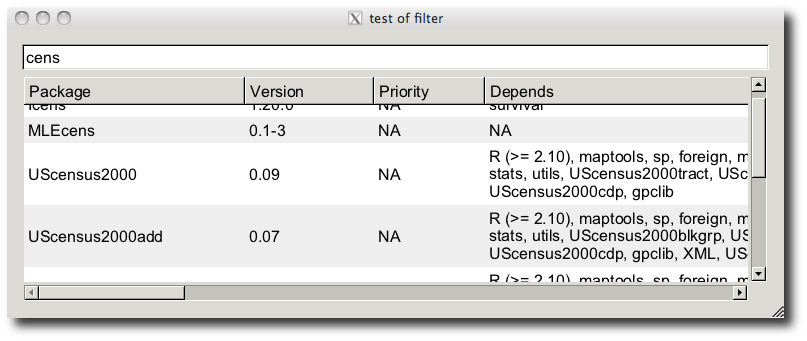
\includegraphics[width=.8\textwidth]{fig-gWidgets-filter-example}
  \caption{Example of using filter to narrow display of tabular data}
  \label{fig:gWidgets-filter-example}
\end{figure}

Even with moderate-sized data sets, the number of rows can be quite large, in which case it is
inconvenient to use a GUI for selection unless some means of searching or filtering the
data is used. This example uses the possible CRAN sites, to show how a
\code{gedit} instance can be used as a search box to filter the display of
data (Figure~\ref{fig:gWidgets-filter-example}). The \code{addHandlerKeystroke} method is used so that the search
results are updated as the user types.


The \code{available.packages} function returns a data frame of all
available packages. If a CRAN site is not set, the user will be
queried to set one.
\begin{Schunk}
\begin{Sinput}
 d <- available.packages()       # pick a cran site
\end{Sinput}
\end{Schunk}

This basic GUI is barebones, for example we skip adding text labels to guide the user. 
\begin{Schunk}
\begin{Sinput}
 w <- gwindow("test of filter")
 g <- ggroup(cont=w, horizontal=FALSE)
 ed <- gedit("", cont=g)
 tbl <- gtable(d, cont=g, filter.FUN="manual", expand=TRUE)
\end{Sinput}
\end{Schunk}
The \argument{filter.FUN}{gtable} provides a means to have a combobox
control the display of the table. For this example, we desire more
flexibility, so we specify the value of \qcode{manual}.

Different search criteria may be desired, so it makes sense to
separate out this code from the GUI code using a function. The one below
uses \code{grep} to match, so that regular expressions can be
used. Another reasonable choice would be to use the first letter of
the package. (That filtering could also be specified easily through the
\argument{filter.FUN}{gtable} argument.)

\begin{Schunk}
\begin{Sinput}
 ourMatch <- function(curVal, vals) {
   ind <- grep(curVal, vals)             # indices
   vis <- rep(FALSE, length(vals))
   if(length(ind) > 0)
     vis[ind] <- TRUE
   return(vis)                           # logical
 }
\end{Sinput}
\end{Schunk}

Finally, the \code{addHandlerKeystroke} method calls its handler
everytime a key is released while the focus is in the edit widget. In
this case, the handler finds the matching indices using the
\code{ourMatch} function, converts these into logical format, and then
updates the display using the \meth{visible\ASSIGN} method for
  \code{gtable}.
\begin{Schunk}
\begin{Sinput}
 id <- addHandlerKeystroke(ed, handler=function(h, ...) {
   vals <- tbl[, 1, drop=TRUE]
   curVal <- svalue(h$obj)
   vis <- ourMatch(curVal, as.character(vals))
   visible(tbl) <- vis
 })
\end{Sinput}
\end{Schunk}
\end{example}


\section{Display of hierarchical data}
\label{sec:gWidgets-displ-heir-data}

The \constructor{gtree} constructor can be used to display
heirarchical structures, such as a file system or the components of a
list. The \constructor{gtree} implementation dynamically computes the
child components, by parameterizing the data to be displayed in terms
of the node of the tree that is currently selected. The
\argument{offspring}{gtree} argument is assigned a function of two
arguments, the path a particular node and the arbitrary object passed
through the optional \argument{offspring.data}{gtree} argument. This
function should return a data frame with each row referring to an
offspring for the node and whose first column is a key that identifies
each of the offspring, unless the argument \argument{chosencol}{gtree}
is used to specify otherwise.

To indicate if a node has offspring, a function can be passed through
the \argument{hasOffspring}{gtree} argument. This function takes the
data frame returned by the \code{offspring} function and should return
a logical vector with each value indicating which rows have
offspring. If it is more convenient to compute this within the
\code{offspring} function, then when \code{hasOffspring} is left
unspecified and the second column returned by \code{offspring} is a
logical, then that column will be used.

As an illustration, this function produces an offspring function to
explore the heirarchical structure of a list. It uses a closure to
encapsulate the list, rather than using the
\argument{offspring.data}{gtree} argument or a global variable.
\begin{Schunk}
\begin{Sinput}
 listOffspring <- function(lst) {
   offspring <- function(path=character(0),...) {
     if(length(path))
       obj <- lst[[path]]
     else
       obj <- lst
     nms <- names(obj)
     hasOffspring <- sapply(nms, function(i) {
       newobj <- obj[[i]]
       is.recursive(newobj) && !is.null(names(newobj))
     })
     data.frame(comps=nms, hasOffspring=hasOffspring, 
                stringsAsFactors=FALSE)
   }
   return(offspring)                     
 }
\end{Sinput}
\end{Schunk}
%
The above will produce a tree with just one column. By adding columns
to the data frame above, say a column to record the class of the
variable, more information can easily be presented

To see the above used, we define a list to explore.
\begin{Schunk}
\begin{Sinput}
 l <- list(a="1", b=list(a="11", b="12", c=list(a="111")))
 o <- listOffspring(l)
 w <- gwindow("Tree test")
 t <- gtree(o, cont=w)
\end{Sinput}
\end{Schunk}
%%


A single click is used to select a row. Multiple selections are
possible if the \argument{multiple}{gtree} argument is given a
\code{TRUE} value.

For some toolkits the \argument{icon.FUN}{gtree} can be used to
specify a stock icon to be displayed next to the first column. This
function, like \code{hasOffspring}, has as an argument the data frame
returned by \code{offspring} and should return a character vector with
each entry indicating which stock icon is to be shown.

For some toolkits, the column type must be determined prior to
rendering. By default, a call to \code{offspring} with argument
\code{c()} indicating the root node is made. The returned data frame
is used to determine the column types. If that is not correct, the
argument \argument{col.types}{gtree} can be used. It should be a data
frame with column types matching those returned by \code{offspring}.

\paragraph{Methods}
The \method{svalue}{gtree} method returns the currently selected key,
or node label. There is no assignment method. The \method{[}{gtree}
method returns the path for the currently selected node. This is what
is passed to the \code{offspring} function.  The
\method{update}{gtree} method updates the displayed tree by
considering the children of the root node.  The method
\method{addHandlerDoubleclick}{gtree} specifies a function to call on
a double click event.

\begin{example}{Using \code{gtree} to explore a recursive partition}{ex-gWidgets-gtree}

The \pkg{party} package implements a recursive partitioning algorithm
for tree-based regression and classification models. The package
provides an excellent \code{plot} method for the object, but in this
example we demonstrate how the \code{gtree} widget can be used to
display the heiarchical nature of the fitted object. As working
directly with the return object, is not for the faint of heart, such a
GUI can be useful.

First, we fit a model from an
example appearing in the package's vignette.

\begin{Schunk}
\begin{Sinput}
 require(party)
 data("GlaucomaM", package="ipred")      # load data
 gt <- ctree(Class ~ ., data=GlaucomaM)  # fit model
\end{Sinput}
\end{Schunk}

The \pkg{party} object tracks the heirarchical nature through its
nodes. This object has a complex structure using lists to store data
about the nodes. We define an \code{offspring} function next that
tracks the node by number, as is done in the \pkg{party} object;
records whether a node has offspring through the \code{terminal}
component (bypassing the \code{hasOffspring} function); and computes a
condition on the variable that creates the node. For this example, the
trees are all binary trees with 0 or 2 offspring so this data frame
has only 0 or 2 rows.

\begin{Schunk}
\begin{Sinput}
 offspring <- function(key, offspring.data) {
   if(missing(key) || length(key) == 0)  # which node?
     node <- 1
   else
     node <- as.numeric(key[length(key)]) # key is a vector
 
   if(nodes(gt, node)[[1]]$terminal)    # return if terminal
     return(data.frame(node=node, hasOffspring=FALSE,
                       description="terminal",
                       stringsAsFactors=FALSE))
 
   df <- data.frame(node=integer(2), hasOffspring=logical(2),
                    description=character(2), 
                    stringsAsFactors=FALSE)
   ## party internals
   children <-  c("left","right")
   ineq <- c(" <= "," >  ")
   varName <- nodes(gt, node)[[1]]$psplit$variableName
   splitPoint <- nodes(gt, node)[[1]]$psplit$splitpoint
 
   for(i in 1:2) {
     df[i,1] <- nodes(gt, node)[[1]][[children[i]]][[1]]
     df[i,2] <- !nodes(gt, df[i,1])[[1]]$terminal
     df[i,3] <- paste(varName, splitPoint, sep=ineq[i])
   }
   df                                    # returns a data frame
 }
\end{Sinput}
\end{Schunk}

\begin{figure}
  \centering
  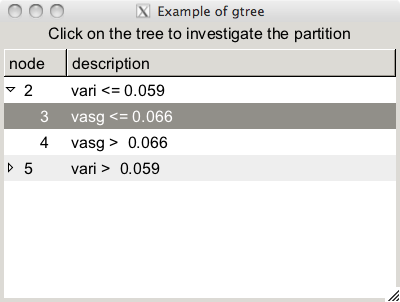
\includegraphics[width=.5\textwidth]{ex-gWidgets-gtree}
  \caption{GUI to explore return value of a model fit by the \code{party}  package.}
  \label{fig:ex-gWidgets-gtree-party}
\end{figure}


We make a simple GUI to show the widget (Figure~\ref{fig:ex-gWidgets-gtree-party})
\begin{Schunk}
\begin{Sinput}
 w <- gwindow("Example of gtree")
 g <- ggroup(cont=w, horizontal=FALSE)
 l <- glabel("Click on the tree to investigate the partition", 
             cont=g)
 tr <- gtree(offspring, cont=g, expand=TRUE)
\end{Sinput}
\end{Schunk}

A single click is used to expand the tree, here we create a binding to
a double click event to create a basic graphic. The \pkg{party}
vignette shows how to make more complicated -- and meaningful --
graphics for this model fit.
\begin{Schunk}
\begin{Sinput}
 addHandlerDoubleclick(tr, handler=function(h,...) {
   node <- as.numeric(svalue(h$obj))
   if(nodes(gt, node)[[1]]$terminal) {   # if terminal plot
     weights <- as.logical(nodes(gt,node)[[1]]$weights)
     plot(response(gt)[weights, ])
   }})
\end{Sinput}
\end{Schunk}
\end{example}





\section{Actions, menus and toolbars}
\label{sec:gWidgets-acti-menus-toolb}

%% ML: Is the overview really the right place for this? As you said,
%% this really needs an example. I think it could go into the control
%% widget chapter, at the end.
%% JV: agreed, moved.

Actions are invisible objects representing an application command that
is executable through one or more widgets. See \ref{sec:GUI:actions}
for more details. Actions in \pkg{gWidgets} are created through the
\constructor{gaction} contstructor. The arguments are
\argument{label}{gaction}, \argument{tooltip}{gaction},
\argument{icon}{gaction}, \argument{key.accel}{gaction} and the
standard \argument{handler}{gaction} and
\argument{action}{gaction}. The label appears as the text on a button,
the menu item or toolbar text, whereas the icon will decorate the same
if possible. For some toolkits, the tooltip pops up when the mouse
hovers.  (See also the \meth{tooltip\ASSIGN} method.)

\paragraph{methods}
The main methods for actions are \method{svalue\ASSIGN}{gaction} to
set the label text and \method{enabled\ASSIGN}{gaction} to adjust
whether the widget is sensitive to user input. All instances of the
action are set through one call. In some toolkits, such as
\pkg{RGtk2}, actions are bundled together into action groups. This
grouping allows one to set the sensitivity of related actions at
once. In \R, one can store like actions in a list, and get similar
functionality by using \code{sapply}, for example.

\paragraph{buttons}
An action can be assigned to a button by setting it as the
\argument{action}{gbutton} argument of the \code{gbutton} constructor,
in which case all other arguments for the constructor are ignored.

\begin{Schunk}
\begin{Sinput}
 w <- gwindow("gaction example")
 a <- gaction("click me", tooltip="Click for a message", icon="ok", 
              handler=function(h,...) {
                print("Hello")
                })
 b <- gbutton(action=a, cont=w)
 ## .. to change
 enabled(a) <- FALSE                     # can't click now
\end{Sinput}
\end{Schunk}
%%
Action handlers generally do not have the sender object (\code{b})
passed back to them. Instead, one uses
the \argument{action}{gaction} argument to parameterize the call.



\subsection{Toolbars}
\label{sec:gWidgets-toolbars}
Toolbars and menubars are implemented in \pkg{gWidgets} using
\code{gaction} items. Toolbars (and menubars) are specified using a named
list of menu components. 

For a toolbar, the list has a simple structure. Each named component
either describes a toolbar item or a separator. The toolbar items are
specified by \code{gaction} instances and separators by
\code{gseparator} instances with no container specified.

For example,
\begin{Schunk}
\begin{Sinput}
 w <- gwindow("gtoolbar example")
 l <- list(Open=gaction("Open", icon="open", 
             handler=function(...) print("Open")),
           Close=gaction("Close", icon="cancel", 
             handler=function(...) print("Close")),
           sep=gseparator(),
           Quit=gaction("Quit", icon="quit", 
             handler=function(...) print("Quit"))
           )
 tb <- gtoolbar(l, cont=w)
 gtext("Placeholder", cont=w)
\end{Sinput}
\end{Schunk}


The \constructor{gtoolbar} constructor takes the list as its first
argument.  As toolbars belong to the window, the corresponding
\pkg{gWigdets} objects use a \constructor{gwindow} object as the
parent container. (Some of the toolkits relax this.)  The argument
\argument{style}{gtoolbar} can be one of \qcode{both}, \qcode{icons},
\qcode{text}, or \qcode{both-horiz} to specify how the toolbar is
rendered. Toolbars in \pkg{gWidgetstcltk} are not native widgets, so
the implementation uses aligned buttons.


\subsection{Menubars, popup menus}
\label{sec:gWidgets-menubars}

Menubars and popup menus are specified in a similar manner as toolbars with menu items
being defined through \code{gaction} instances, and visual separators
by \code{gseparator} instances. Menus differ from toolbars, as
submenus require a nested structure. This  is specified using a
nested list as the component to describe the sub menu. The lists all
have named components. In this case, the corresponding name is used to
label the submenu item. For menu bars, it is typical that all the
top-level components be lists, but for popup menus, this wouldn't
necessarily be the case.

A example of such a list might be
\begin{Schunk}
\begin{Sinput}
 f <- function(h,...) print(h$action)                # a stub
 ml <- list(File=list(
              Source=gaction("Source file...", action="source",  
                handler=f),
              Load=gaction("Load workspace...", action="load", 
                handler=f),
              sep=gseparator(),
              New=list(
                Plot=gaction("Plot window", action="plot", 
                  handler=f),
                Rfile=gaction("R file", action="file", handler=f)
                )
              ),
            Help=list(
              about=gaction("About", action="about", handler=f)
              )
            )
\end{Sinput}
\end{Schunk}

\begin{Schunk}
\begin{Soutput}
guiWidget of type: gTextRGtk for toolkit: guiWidgetsToolkitRGtk2 
\end{Soutput}
\end{Schunk}


In Mac OS X, with a native toolkit, menubars may be drawn along the top
of the screen, as is the custom of that OS. 

\paragraph{Menubar and Toolbar Methods}
The main methods for toolbar and menubar instances are
the \method{svalue}{gmenu} method which will return the list. Whereas, the
\method{svalue\ASSIGN}{gmenu} method can be used to redefine the
menubar or toolbar. Use the \method{add}{gmenu} method to append to an
existing menubar or toolbar, again using a list to specify the new items.


% \begin{example}{Menubar and toolbar example}{ex-gWidgets-menu-tool-status-bars}
%   \SweaveInput{ex-gWidgets-menu-tool-status-bars}
% \end{example}

\paragraph{Popup menus}

Popup menus can be created for a right click event through the
\constructor{add3rdMousePopupmenu} constructor. (Or
\kbd{control-button-1} for Mac OS X.) This constructor has arguments
\code{obj} to specify a widget, like a button, to initiate the popup,
\argument{menulist}{gmenu} to specify the menu and optionally an
\argument{action}{gmenu} argument.


\begin{example}{Popup menus}{ex-gWidgets-context-menus}
\begin{Schunk}
\begin{Sinput}
 w <- gwindow("Popup example")
 b <- gbutton("click me or right click me", cont=w, 
              handler=function(h, ...) {
                cat("You clicked me\n")
              })
 f <- function(h,...) cat("you right clicked on", h$action)
 mbList <- list(one = gaction("one", action="one", handler=f),
                two = gaction("two", action="two", handler=f)
                )
 add3rdMousePopupmenu(b, mbList)
\end{Sinput}
\end{Schunk}

\end{example}












\chapter{\pkg{gWidgets}: R-specific  widgets}
\label{cha:compound-widgets}
The \pkg{gWidgets} package provides some \R\/ specific widgets for
producing GUIs. Table~\ref{tab:gWidgets-compound-widgets} lists them.


\begin{table}
\centering
\label{tab:gWidgets-compound-widgets}
\caption{Table of constructors for compound widgets in \pkg{gWidgets}}
\begin{tabular}{@{}lp{0.7\textwidth}@{}}
\toprule

Constructor&Description\\
\midrule
\constructor{gvarbrowser}&GUI for browsing variables in the workspace\\\constructor{gcommandline}&Command line widget\\\constructor{gformlayout}&Creates a GUI from a list specifying layout\\\constructor{ggenericwidget}&Creates a GUI for a function based on its formal arguments or a defining list
\\ \bottomrule
\end{tabular}
\end{table}
% \begin{table}
%   \centering
%   \begin{tabular}{l@{\quad}p{.75\textwidth}}
% %    \toprule
%     \constructor{gcommandline} & Command line widget\\ 
%     \constructor{gvarbrowser} & GUI for browsing variables in the workspace\\
% %    \constructor{gdfnotebook} & A notebook of data frames\\
% %    \constructor{ggraphicsnotebook} & A notebook for graphics objects\\
%     \constructor{ghelp} & GUI for a help page\\
%     \constructor{ghelpbrowser} & A help browser\\
%     \constructor{gformlayout} & Uses list to specify layout of a GUI\\
%     \constructor{ggenericwidget} & Creates a GUI for a function based
%     on its formal arguments or a defining list\\
%     \bottomrule
%   \end{tabular}
%   \caption{Table of compound widgets provided by \pkg{gWidgets}}
%   \label{tab:gWidgets-compound-widgets}
% \end{table}


\section{A graphics device}
\label{sec:gWidgets-graphics-device}

Some toolkits support an embeddable graphics device (\pkg{gWidgetsRGtk2}
through \pkg{cairoDevice}, \pkg{gWidgetsQt} through \pkg{qtutils}). In which case, the \constructor{ggraphics}
constructor produces a widget that can be added to a container. The
arguments \argument{width}{ggraphics}, \argument{height}{ggraphics},
\argument{dpi}{ggraphics}, \argument{ps}{ggraphics} are similar to
other graphics devices.

%% current device
When working with multiple devices, it becomes necessary to switch
between devices. A \code{ggraphics} instance can be made to represent the
current device if the user clicks in the window. Otherwise, the
\method{visible\ASSIGN}{ggraphics} method can be used to set the
object as the current device.

%% handlers
The default handler for the widget is set by
\method{addHandlerClicked}{ggraphics}. The coordinates of the mouse
click, in user coordinates, are passed to the handler in the
components \code{x} and \code{y}. As well, the method
\method{addHandlerChanged}{ggraphics} is used to assign a handler to
call when a region is selected by dragging the mouse. The components
\code{x} and \code{y} describe the rectangle that was traced out,
again in user coordinates.

\begin{Schunk}
\begin{Sinput}
 w <- gwindow("ggraphics example")
 g <- ggraphics(cont=w)
 x <- mtcars$wt; y <- mtcars$mpg
 #
 addHandlerClicked(g, handler=function(h,...) {
   cat(sprintf("You clicked %s x %s\n", h$x, h$y))
 })
 addHandlerChanged(g, handler=function(h,...) {
   rx <- h$x; ry <- h$y
   if(diff(rx) > diff(range(x))/100 && 
      diff(ry) > diff(range(y))/100) {
     ind <- rx[1] <= x & x <= rx[2] & ry[1] <=y & y <= ry[2]
     if(any(ind))
       print(cbind(x=x[ind], y=y[ind]))
   }
 })
 #
 plot(x, y)
\end{Sinput}
\end{Schunk}
%

The \constructor{ggraphicsnotebook} creates a notebook that allows the
user to easily navigate multiple graphics devices.




%% XXXX Move this example somewhere COMPONENT PROGRAMMING
\begin{example}{A GUI for filtering and visualizing a data set}{ex:gWidgets-spotfire}
%% Example of a spotfire like interface

\begin{figure}
  \centering
  \includegraphics[width=.6\textwidth]{fig-gWidgets-spotfire-gui}
  \caption{A GUI to filter a data frame and display an accompanying graphic.}
  \label{fig:gWidgets-spotfire-gui}
\end{figure}
A common GUI applicatio
n for data analysis consists of means to
visualize, query, aggregate and filter a data set. This example shows
how one can create such a GUI using \pkg{gWidgets} featuring
an embedded graphics device. In addition a visual display of the filtered data,
and a means to filter, or narrow, the data that is under
consideration, is presented (Figure~\ref{fig:gWidgets-spotfire-gui}).
Although, our example is not too feature rich, it illustrates a
framework that can easily be extended.


This example is centered around filtering a data set, we choose a
convenient one and give it a non-specific name.
\begin{Schunk}
\begin{Sinput}
 data("Cars93", package="MASS")
 x <- Cars93
\end{Sinput}
\end{Schunk}

We use a notebook to hold two tabs, one to give information and one
for the main GUI. This basic design comes from the spotfire demos at \url{tibco.com}.
\begin{Schunk}
\begin{Sinput}
 w <- gwindow("Spotfire example", visible=FALSE)
 nb <- gnotebook(cont=w)
\end{Sinput}
\end{Schunk}


We use a simple label for information, although a more detailed
description would be warranted in an actual application.

\begin{Schunk}
\begin{Sinput}
 descr <- glabel(gettext("A basic GUI to explore a data set"), 
                 cont=nb, label=gettext("About"))
\end{Sinput}
\end{Schunk}
%
Now we specify the layout for the second tab. This is a nested layout
made up of three box containers. The first, \code{g}, uses a
horizontal layout in which we pack to box containers that will use a
vertical layout (when \code{horizontal=FALSE}). 

\begin{Schunk}
\begin{Sinput}
 g <- ggroup(cont=nb, label=gettext("Explore..."))
 lg <- ggroup(cont=g, horizontal=FALSE) # vertical boxes
 rg <- ggroup(cont=g, horizontal=FALSE)
\end{Sinput}
\end{Schunk}

The left side will contain an embedded graphic device and a view of
the filtered data. The \constructor{ggraphics} widget provides the
graphic device. This widget is unfortunately not available for all toolkits
\begin{Schunk}
\begin{Sinput}
 ggraphics(cont = lg)
\end{Sinput}
\begin{Soutput}
guiWidget of type: gGraphicsRGtk for toolkit: guiWidgetsToolkitRGtk2 
\end{Soutput}
\end{Schunk}

Our view of the data is provided by the \constructor{gtable} widget,
which facilitates the display of a data frame. The last two arguments
allow for multiple selection (for marking points on the graphic) and
for filtering through the \method{visible\ASSIGN}{gtable} method.
In addition to the table, we add a label to display the number of
cases being shown. This label is packed into a box container, and
forced to the right side through the \method{addSpring}{ggroup} method
of the box container.
\begin{Schunk}
\begin{Sinput}
 tbl <- gtable(x, cont = lg, multiple=TRUE, filter.FUN="manual")
 size(tbl) <- c(500, 200)                # set size
 labelg <- ggroup(cont = lg)
 addSpring(labelg)
 noCases <- glabel("", cont = labelg)
\end{Sinput}
\end{Schunk}

The right panel is used to provide the user a means to filter the
display. We place the widgets used to do this within a frame to guide
the user.
\begin{Schunk}
\begin{Sinput}
 filterg <- gframe(gettext("Filter by:"), cont = rg, expand=TRUE)
\end{Sinput}
\end{Schunk}
The controls are layed out in a grid. We have two here to filter by
type and the number of cylinders. These of course, are specific to the
data set.
\begin{Schunk}
\begin{Sinput}
 lyt <- glayout(cont=filterg)
 l <- list() # store widgets
 lyt[1,1] <- "Type:"
 lyt[1,2] <- (l$Type <- gcombobox(c("", levels(x$Type)), cont=lyt))
 lyt[2,1] <- "Cylinders:"
 lyt[2,2] <- (l$Cylinders <- gcombobox(c("", levels(x$Cylinders)), cont=lyt))
\end{Sinput}
\end{Schunk}
%
Of course, we could use many more criteria to filter. The above
filters are naturally represented by a combobobox. However, one could
have used many different styles, depending on the type of data. For
instance, one could employ a checkbox to filter through Boolean data,
a slider to pick out numeric data, or a text box to specify a
filtering by a string. The type of data dictates this.

%% handlers
There are three main components in our GUI: the display, the table and
the filters. We create handlers to connect these components. This
first handler is used to
update the data frame when the filter controls are changed. For this
we need to compute a logical variable indicating which rows are to be
considered.  Within the definition of the function, we use the global
variables \code{l}, \code{tbl} and \code{noCases}.
\begin{Schunk}
\begin{Sinput}
 updateDataFrame <- function(...) {
   ind <- rep(TRUE, nrow(x))
   for(i in c("Type", "Cylinders"))  {
     if((val <- svalue(l[[i]])) != "") 
       ind <- ind & (x[,i] == val)
   }
   
   visible(tbl) <- ind                   # udpate table
   
   nsprintf <- function(n, msg1, msg2,...)
     ngettext(n, sprintf(msg1, n), sprintf(msg2,n), ...)
   svalue(noCases) <- nsprintf(sum(ind), "%s case", "%s cases") # label
 }
\end{Sinput}
\end{Schunk}

% %% methods
% The \method{visible\ASSIGN}{gtable} and \method{svalue\ASSIGN}{glabel}
% methods change the underlying widgets. The generic
% \meth{svalue\ASSIGN} is used to change the primary value for a widget
% (and \meth{svalue} returns this value). In the above, we see these
% methods used to get the values from the comboboxes and to set the text
% in the label. The \meth{visible\ASSIGN} method is another generic. In
% this example it is used to specify which rows of the data are actually
% displayed by the widget.

This next function is used to update the graphic. Of course, this graphic is not
so interesting, but in a real application, it should be.
\begin{Schunk}
\begin{Sinput}
 updateGraphic <- function(...) {
   ind <- visible(tbl)
   if(any(ind))
     plot(MPG.city ~ Weight, data=x[ind,])
   else
     plot.new()
 }
\end{Sinput}
\end{Schunk}

We now add a handler to be called whenever one of our comboboxes is
changed. This handler simply calls both our update functions.
\begin{Schunk}
\begin{Sinput}
 f <- function(h, ...) {
   updateDataFrame()
   updateGraphic()
 }
 sapply(l, function(i) addHandlerChanged(i, handler=f))
\end{Sinput}
\begin{Soutput}
     Type.changed Cylinders.changed 
             2681              2682 
\end{Soutput}
\end{Schunk}
%
For the data display, we wish to allow the user to view individual cases
by clicking on a row of the table. The following will do so.

\begin{Schunk}
\begin{Sinput}
 addHandlerClicked(tbl, handler=function(h,...) {
   updateGraphic()
   ind <- svalue(h$obj, index=TRUE)
   points(MPG.city ~ Weight, cex=2, col="red", pch=16, data=x[ind,])
 })
\end{Sinput}
\end{Schunk}
%
We could also use the \method{addHandlerChanged}{ggraphics} method to
add a handler to call when the user drags our a region in the graphics
device, but leave this for the interested reader.


Finally, we draw the GUI with an initial graphic (the
\method{visible}{gwindow} method draws the GUI here, unlike its use
with \code{gtable}).
\begin{Schunk}
\begin{Sinput}
 visible(w) <- TRUE
 updateGraphic()
\end{Sinput}
\end{Schunk}
\end{example}

%%% 
% \begin{example}{A GUI to explore a data set}{ex-gWidgets-baseball}
%   \SweaveInput{ex-gWidgets-baseball-RGtk2.Rnw}
% \end{example}


\section{A data frame editor}
\label{sec:gWidgets-an-editor-tabular}

The \constructor{gdf} constructor returns a widget for editing data
frames. The intent is to produce a toolkit widget atleast as powerful
as the \function{data.entry} function. The implementations differ
between toolkits, with some offering much more. We describe what is in
common below, but note that some toolkits have popup menus allowing
much more.~\footnote{ For \pkg{gWidgetstcltk}, there is no native
  widget for editing tabular data, so the \code{tktable} add-on widget
  is used (\url{tktable.sourceforge.net}). A warning will be issued if
  this is not installed. For \pkg{gWidgetsRGtk2} there is also the
  \constructor{gdfedit} constructor which is faster and has many improved
  usability features. The \pkg{gWidgets} function merely wraps the \function{gtkDfEdit}
  function from \pkg{RGtk2Extras}. This function is not exported by
  \pkg{gWidgets}, so the toolkit package must be loaded. Again, as
  with \function{gtable}, the widget under \pkg{gWidgetstcltk} is
  slower, can load a moderately sized data frame in a reasonable
  time. }


The constructor has its main argument \argument{items}{gdf} to specify the data
frame to edit. A basic usage might be:

\begin{Schunk}
\begin{Sinput}
 w <- gwindow("gdf example")
 df <- gdf(mtcars, cont=w)
 ## ... make some edits ...
 newDataFrame <- df[,]                   # store changes
\end{Sinput}
\end{Schunk}
%

Some toolkits render columns differently for different data types, and
some toolkits use character values for all the data, so values must be
coerced back when transferring to \R\/ values. As such, column types
are important. Even if one is starting with a $0$-row data frame, the
columns types should be defined as desired. Also, factors and
character types may be treated differently, although they may render
in a similar manner.

\paragraph{Methods} The \method{svalue}{gdf} method will return the
selected values or selected indices if \code{index=TRUE} is
given. The \method{svalue\ASSIGN}{gdf} method is used to specify the
selection by index. This is a vector, or for some toolkits a list with
components \code{rows} and \code{columns} indicating the selection to
mark.  The \method{[}{gdf} and \method{[\ASSIGN}{gdf} methods can be
used to extract and set values from the data frame by index. As with
\code{gtable}, these are not as flexible as for a data frame. In
particular, it may not be possible to change the type of a column, or
add new rows or columns through these methods. Using no indices, as in
the above example with \code{df[,]}, will return the current data
frame. The current data frame can be completely replaced, when no
indices are specified in the replacement call. 

There are also several methods defined that follow those of a data
frame: \method{dimnames}{gdf}, \method{dimnames\ASSIGN}{gdf},
\method{names}{gdf}, \method{names\ASSIGN}{gdf}, and
\method{length}{gdf}.

The following methods can be used to assign handlers (all are
implemented in \pkg{gWidgetsRGtk2}, but not for the others):
\method{addHandlerChanged}{gdf} (cell changed),
\method{addHandlerClicked}{gdf}, \method{addHandlerDoubleclick}{gdf},
\method{addHandlerColumnClicked}{gdf},
\method{addHandlerColumnDoubleclick}{gdf}, and
\method{addHandlerColumnRightclick}{gdf}.
\\


The \constructor{gdfnotebook} constructor produces a notebook that can
hold several data frames to edit at once.





\subsection{Workspace browser}
\label{sec:gWidgets-workspace-browser}

A workspace browser is constructed by \code{gvarbrowser}, providing a
means to browse and select the objects in the current global
environment. This workspace browser uses a tree widget to display the
items and their named components, if applicable.

The default \argument{handler}{gvarbrowser} object calls
\code{do.call} on the object for the function specified by name
through the \argument{action}{gvarbrowser} argument. (The default is
to print a \code{summary} of the object.) This handler is called on a
double click. A single click is used for selection. One can pass in
other handler functions if desired.  The name of the currently
selected value is returned by the \method{svalue}{gvarbrowser} method.


The \method{update}{gvarbrowser} method will update the list of items
being displayed.  As, \R\/ has no means to notify observers if its
global workspace exists, the user can either invoke this method, or
have the GUI poll every so often to query
for changes (\meth{addHandlerIdle}). As the latter can be time consuming if there are many objects
in the global environment, it isn't implemented in for each toolkit.

\begin{example}{Using drag and drop with \pkg{gWidgets}}{ex-gWidgets-drag-and-drop}
  We use the drag and drop features to create a means to plot
  variables from the workspace browser.  Our basic layout is fairly
  simple. We place the workspace browser on the left, and on the right
  have a graphic device and few labels to act as drop targets.
\begin{Schunk}
\begin{Sinput}
 w <- gwindow("Drag and drop example")
 g <- ggroup(cont=w)
 vb <- gvarbrowser(cont=g)
 g1 <- ggroup(horizontal=FALSE, cont=g, expand=TRUE)
 ggraphics(cont=g1)
\end{Sinput}
\begin{Soutput}
guiWidget of type: gGraphicsRGtk for toolkit: guiWidgetsToolkitRGtk2 
\end{Soutput}
\begin{Sinput}
 xlabel <- glabel("", cont=g1)
 ylabel <- glabel("", cont=g1)
 clear <- gbutton("clear", cont=g1)
\end{Sinput}
\end{Schunk}
%
We create a function to initialize the interface.
\begin{Schunk}
\begin{Sinput}
 init_txt <- "<Drop %s variable here>"
 initUI <- function(...) {
   svalue(xlabel) <- sprintf(init_txt, "x")
   svalue(ylabel) <- sprintf(init_txt, "y")
   enabled(ylabel) <- FALSE
 }
 initUI()                                # initial call
\end{Sinput}
\end{Schunk}
%
Separating this out allows us to link it to the clear button.
\begin{Schunk}
\begin{Sinput}
 addHandlerClicked(clear, handler=function(h,...) {
   initUI()
 })
\end{Sinput}
\end{Schunk}
%
Next, we write a function to update the user interface. In this case
we need to figure out which state the GUI is currently in by
considering the text in each drop label.
\begin{Schunk}
\begin{Sinput}
 updateUI <- function(...) {
   if(grepl(svalue(xlabel), sprintf(init_txt, "x"))) {
     ## none set
     enabled(ylabel) <- FALSE
   } else if(grepl(svalue(ylabel), sprintf(init_txt, "y"))) {
     ## x, not y
     enabled(ylabel) <- TRUE
     x <- eval(parse(text=svalue(xlabel)), envir=.GlobalEnv)
     plot(x, xlab=svalue(xlabel))
   } else {
     enabled(ylabel) <- TRUE    
     x <- eval(parse(text=svalue(xlabel)), envir=.GlobalEnv)
     y <- eval(parse(text=svalue(ylabel)), envir=.GlobalEnv)
     plot(x, y, xlab=svalue(xlabel), ylab=svalue(ylabel))
   }
 }
\end{Sinput}
\end{Schunk}

Now we add our drag and drop information.  Drag and drop support in
\pkg{gWidgets} is implemented through three methods: one to set a
widget as a drag source (\generic{addDropSource}), one to set a widget
as a drop target (\generic{addDropTarget}), and one to call a handler
when a drop event passes over a widget (\generic{addDropMotion}).
  

The \generic{addDropSource} method needs a widget and a handler to
call when a drag and drop event is initiated. This handler should
return the value that will be passed to the drop target. The default
value is that returned by calling \code{svalue} on the object. In this
example we don't need to set this, as \generic{gvarbrowser} already
calls this with a drop data being the variable name using the dollar
sign notation for child components.
    
The \generic{addDropTarget} method is used to allow a widget to
receive a dropped value and to specify a handler to call when a value
is dropped. The \code{dropdata} component of the first callback
argument, \code{h}, holds the drop data. In our example below we use
this to update the receiver object, either the $x$ or $y$ label.

\begin{Schunk}
\begin{Sinput}
 dropHandler <- function(h,...) {
   svalue(h$obj) <- h$dropdata
   updateUI()
 }
 addDropTarget(xlabel, handler=dropHandler)
 addDropTarget(ylabel, handler=dropHandler)
\end{Sinput}
\end{Schunk}


The \generic{addDropMotion} registers a handler for when a drag event
passes over a widget. We don't need this for our GUI.
    
\end{example}



\subsection{Help browser}
\label{sec:gWidgets-help-browser}

The \constructor{ghelp} constructor produces a widget for showing help
pages using a notebook container. Although \R\/ has the excellent
ways to dynamically view help pages through a web browser (in
particuluar the \pkg{helpr} package and the standard built-in help
page server) this widget provides an alternative.

To add a help page, the \method{add}{ghelp} method is used,
where the \code{value} argument describes the desired page. This can
be a character string containing the topic, a character string of the
form \code{package:::topic} to specify the package, or a list with
named components \code{package} and \code{topic}.  The
\method{dispose}{ghelp} method of notebooks can be used to remove the
current tab.
\\

The \constructor{ghelpbrowser} constructor produces a stand-alone
GUI for displaying help pages, running examples from the help pages or
opening vignettes provided by the package. This GUI provides its own
top-level window and does not return a value for which methods are defined.



\subsection{Command line widget}
\label{sec:gWidgets-command-line-widget}



A simple command line widget is created by the
\constructor{gcommandline} constructor. This is not meant as a
replacement for any of \R's commandlines, but is provided for
lightweight usage. A text box allows users to to type in \R\/
commands. The programmer may issue commands to be evaluated and
displayed through the \method{svalue\ASSIGN}{gcommandline} method. The
\code{value} assigned is a character string holding the commands. If
there is a names attribute, the results will be assigned to a variable
in the global workspace with that name. The \code{svalue} and \code{[}
methods return the command history.

\subsection{Simplifying creation of dialogs}
\label{sec:gWidgets-designing-forms}

The \pkg{gWidgets} package has two means to simpify the creation of
GUIs.~\footnote{The \pkg{traitr} package provides another, but is not
  discussed here.} The \code{gformlayout} constructor takes a list defining a
layout and produces a GUI, the \code{ggenericwidget} constructor can
take a function name and produce a GUI based on the formal arguments
of the function. This too uses a list, which can be modified by the
user before the GUI is constructed. 

\subsubsection{Laying out a form}
\label{sec:gWidgets-laying-out-form}

% ML: replaced 'component' with 'element' for components of list, to
% distuingish them from components of the GUI

% ML: this is another place where it would be good to see the example first
%% JV: Good ideas, done.

The \constructor{gformlayout} constructor takes a list defining a
layout and creates the specified widgets. The design borrows from the
\code{extjs} javascript libraries for web programming, where a similar
function can be used to specify the layout of web forms. Several
toolkits have a means to specify a layout using XML (eg. \GTK{}
Builder and \Qt{} Assistant); this implementation uses a list, under
the assumption that it is more familiar to the \R\/ user. By defining
the layout ahead of time, pieces of the layout can be recycled for
other layouts.

A simple example would be
\begin{Schunk}
\begin{Sinput}
 l <- list(type="ggroup",
           horizontal=TRUE,
           children=list(
             list(type="glabel",
                  text="x:"),
             list(name="x",
                  label="asdfas",
                  type="gedit",
                  text="initial text"),
             list(type="glabel",
                  text="state:"),
             list(name="y",
                  type="gcombobox",
                  items=state.name)
             )
           )
 w <- gwindow("glayout example")
 f <- gformlayout(l, cont=w)
\end{Sinput}
\end{Schunk}


To define the layout, each list element is specified using a 
named. The \code{type} element indicates the component
to be created, as a string. This can be the name of a container
constructor, a widget constructor or the special value
\code{"fieldset"}. Field sets are used to group a set of common
controls. 

The list defining each GUI component has named elements to pass to the
constructor, such as \code{text} and \code{items} in the above
example, and named elements used by the \generic{gformlayout}
constructor. For example, 
the \code{name} element when specified, allows that
component to be referenced through \method{svalue}{gformlayout},
which returns the form's values in a list, or \method{[}{gformlayout},
which returns the components in a list.

If the type is a container or fieldset, then the \code{children}
element is a list whose elements specify the children as
above. Except for fieldsets, these children can contain other
containers or controls. Fieldsets only allow controls as children.


%% fields set and labels.
For \code{fieldset}s the \code{label} element adds a descriptive label
to the layout. The \code{label.pos} element controls the placement of
the label. The value \code{"top"} places the label on top of the
widget, while \code{"side"}, the default, puts it on the side. The
\code{label.font} element specifies the font properties of the label,
as with the \meth{font\ASSIGN} method.

Parts of the form can be made to depend on other parts. For example, 
whether a component is enabled or not may be controlled by the by \code{depends.on},
\code{depends.FUN}, and \code{depends.signal} elements. If the
\code{depends.on} element specifies the name of a previous component,
then the function \code{depends.FUN} will be consulted when the signal
specified by \code{depends.signal} is emitted. This uses the
\code{addHandlerXXX} names with a default value of
\code{addHandlerChanged}. The \code{depends.FUN} function should take a single
argument consisting of the value returned by \code{svalue} when called
on the widget specified through \code{depends.on}. This function
should return a logical indicating if the widget is enabled or not.

The constructor returns an object with just a few methods. In addition to
\meth{svalue} and \meth{[}, the \method{names}{gformlayout} method
returns the names of the widgets in the list.

%% JV: this example will be in the package, but perhaps not needed here.
% \begin{example}{The \code{gformlayout} constructor}{ex-gWidgets-gformlayou}
%   \SweaveInput{ex-gWidgets-formlayout}
% \end{example}

\subsubsection{Creating a GUI for a function}
\label{sec:gWidgets-autom-creat-gui}

The \constructor{ggenericwidget} constructor creates a GUI for
invoking a given function. The GUI is derived from the formal
arguments. The \pkg{fgui} package provides a similar function, with
some more features, although limited to the \pkg{tcltk} toolkit.


The usage is straightforward. To make a GUI for a function is as
simple as:
\begin{Schunk}
\begin{Sinput}
 f <- function(x=1, variable="a") {
   print("Something with x and variable")
 }
 g <- ggenericwidget(f, cont=gwindow())
\end{Sinput}
\end{Schunk}
%
The formal arguments of an S3 method may be different from those of
its generic. For instance, those for the \code{t.test} generic are
much different (and less useful for this purpose) than the
\code{t.test.default} method for numeric values for \code{x}. Knowing
this, a useful GUI can be quickly created for the \code{t.test} with
the commands:
\begin{Schunk}
\begin{Sinput}
 w <- gwindow("t.test through ggenericwidget")
 f <- stats:::t.test.default; 
 widget <- ggenericwidget("f", cont=w)
\end{Sinput}
\end{Schunk}


The implementation has two stages. The first creates a list
specifying the layout of the GUI and the second actually constructs
the GUI. This list is different from that used by \code{gformlayout}. It
does not provide as much flexibility and is described in the help page
for \code{ggenericwidget}. This list can dumped to a text file, edited if desired and then
sourced in later. For example:

\begin{Schunk}
\begin{Sinput}
 tmp <- tempfile()
 cat(gWidgets:::autogenerategeneric(f), file=tmp)
 ## ... do some edits ...
 source(tmp)
 w <- gwindow("Another ggeneric widget example")
 ggenericwidget(f.LIST, cont=w)          # made by autogenerategeneric
\end{Sinput}
\end{Schunk}



\XXX{Need to have an example with drag and drop}


%\section{End of chapter notes}
%\label{sec:gWidgets:eoc}





